% ============================================================================
%  PART III: Using, testing and extending
% ============================================================================

\chapter{Installing and Running}
\label{ch:running}

\section{What you need}

\begin{itemize}
  \item \textbf{Python 3.10+} for the backend (developed on 3.14; the Docker image uses 3.12).
  \item \textbf{Node.js 20+} and npm for the frontend.
  \item \textbf{Icarus Verilog 12} (\code{iverilog} and \code{vvp}) on the PATH. On macOS: \code{brew install icarus-verilog}; on Ubuntu: \code{sudo apt install iverilog}.
  \item For live models: the \textbf{OpenCode app}, installed and signed in with your own account. Optionally a Cloudflare account and an NVIDIA NIM key (Section~\ref{sec:providers}). Without any of these, the app runs in offline demo mode.
  \item For the timing and area estimate (optional): \textbf{Yosys} (the WebAssembly build from \code{yowasp-yosys}, reached through a \code{yosys} shim in \file{~/.local/bin}), \textbf{OpenSTA} built with \file{backend/tools/build_opensta.sh} (reached as \code{sta}), and the sky130 library file. Without them the result simply has no timing section.
  \item Optional: Verilator (better linting).
\end{itemize}

\section{First-time setup}

\begin{lstlisting}[style=plain]
cd ai-eda-playground/backend
python3 -m venv venv
source venv/bin/activate
pip install -r requirements.txt

# the sky130 cell library for timing (12 MB, not in git)
cd pdk
curl -fsSL -o sky130hd_tt.lib.gz https://raw.githubusercontent.com/parallaxsw/OpenSTA/master/examples/sky130hd_tt.lib.gz
gunzip -kf sky130hd_tt.lib.gz

cd ../../frontend
npm install
\end{lstlisting}

\section{Starting the app}

The live set-up uses two terminals. Terminal 1 starts the backend with the OpenCode app as the model provider; terminal 2 starts the frontend. The \code{PATH} addition makes \code{yosys}, \code{sta} and Icarus in \file{~/.local/bin} visible; \code{env -u OFFLINE_MODE} makes sure an old offline setting is not inherited.

\begin{lstlisting}[style=plain]
# terminal 1: backend, live model
cd ai-eda-playground/backend
PATH="$HOME/.local/bin:$PATH" env -u OFFLINE_MODE LLM_PROVIDER=opencode-app \
  LLM_MODEL=deepseek-v4.1-flash-free LLM_TIMEOUT_SECONDS=360 \
  python3 -m uvicorn main:app --host 127.0.0.1 --port 8000

# terminal 2: frontend
cd ai-eda-playground/frontend && npm run dev -- --host 127.0.0.1 --port 5173
\end{lstlisting}

Open \url{http://127.0.0.1:5173}. The badge at the top left must say \textbf{Live} followed by a model name (for example \texttt{Live \textbullet\ opencode/deepseek-v4.1-flash-free}); it follows the model chosen in the Model menu. If it says \emph{Offline demo} or \emph{Demo fallback}, the live model is not in use. During development Vite forwards \code{/api} calls to port 8000.

From the project folder, \code{./run.sh} still starts both halves in one terminal (backend on port 8000, frontend on 5173; Ctrl-C stops both), using whatever is in \file{backend/.env}.

\section{Offline mode and live mode}

\begin{description}
  \item[Offline] Set \code{OFFLINE_MODE=1} (or configure nothing). The five built-in designs are used; everything else (simulation, waveforms, repair loop, strength, timing, projects) works for real. The badge shows ``Offline demo'' and the Model menu says ``Offline demo: scripted designs, no AI model.'' The ``Buggy counter'' example is scripted only here: it shows a failure and a repair.
  \item[Live] \code{LLM_PROVIDER=opencode-app} with a default \code{LLM_MODEL}, as above. The default is only where the Model menu starts: any model can be picked per run. Free models are slow: a live run took 3 to 13 minutes in the evaluation (median 360 s), so a generous \code{LLM_TIMEOUT_SECONDS} helps.
\end{description}

\section{Optional providers: Cloudflare, NVIDIA NIM and GitHub Copilot}
\label{sec:providers}

The Model menu has three tabs. OpenCode works as soon as the app is signed in. The other two need a key, and keys go in exactly one place: the file \file{backend/.env}.

\begin{lstlisting}[style=plain]
# backend/.env  (git-ignored; keep it owner-only:  chmod 600 backend/.env)
CLOUDFLARE_ACCOUNT_ID=your_32_character_account_id
CLOUDFLARE_API_TOKEN=your_workers_ai_token
NVIDIA_NIM_API_KEY=nvapi-your_key_here
\end{lstlisting}

\begin{description}
  \item[Cloudflare Workers AI] Needs your account id (32 hexadecimal characters) and an API token with the ``Workers AI'' permission. The free plan gives 10,000 ``neurons'' a day. Some models are refused on the free plan (HTTP 403, code 5035, seen for GLM-5.3-flash and DeepSeek V4.1 Flash).
  \item[NVIDIA NIM] Needs a key that starts with \code{nvapi-}. Only \code{NVIDIA_NIM_API_KEY} is read for this tab; an older \code{NVIDIA_API_KEY} is never used for it. The fastest chat models answered in about 1 to 7 seconds; some free-queue models took 1 to 5 minutes.
  \item[GitHub Copilot] Is not configured in SiliconScribe at all. Connect it inside the OpenCode app: start \code{opencode} in a terminal, type \code{/connect}, choose GitHub Copilot and sign in with GitHub in the browser. Then press the refresh button next to the source tabs in SiliconScribe. It appears on the OpenCode tab as \code{github-copilot/auto}; because its name is not marked free, tick ``Show other models'' to see it. On the student plan only ``auto'' exists: GitHub picks the model and does not say which, so the result cannot name its model.
\end{description}

Restart the backend after editing \file{.env}. Without the keys, the Cloudflare and NVIDIA NIM tabs say they are not set up and how to fix it; nothing else changes. Delete the lines (or the file) to switch them off.

\begin{warnbox}[Keys: one place only]
Never paste a key into the web page, a prompt, a chat, a screenshot, a document or a commit. The web page never asks for one. Never commit \file{backend/.env}: it is listed in \file{.gitignore}, and the project was scanned to check that no secret is in git, in the built frontend or in the logs. The simulator, synthesis and timing tools receive a scrubbed environment, so the keys never reach them either.
\end{warnbox}

\section{Docker and deployment}

\begin{itemize}
  \item \code{docker compose up --build} builds one image (frontend compiled into \file{static/}, backend with Icarus and Yosys installed) and serves everything on port 8000, offline by default.
  \item The earlier public deployment split the halves: the frontend on Vercel (\file{vercel.json} forwards \code{/api/*} to the backend) and the backend container on Render's free plan (\file{render.yaml}, health check on \code{/health}, \code{TRUST_PROXY_HEADERS=1}). The free backend sleeps after 15 minutes idle, so the first request can take 30--50 seconds. Note that the backend now accepts browser calls only from local addresses unless the exact frontend address is added with \code{CORS_ALLOW_ORIGINS}, and the OpenCode app provider is a single-user, local convenience that must not be exposed on a public server.
\end{itemize}

% ---------------------------------------------------------------------------
\chapter{Using the Application}
\label{ch:usage}

\section{The screen}

The page has three parts. The \textbf{top bar} has the badge on the left (``Live'' with the model chosen in the menu, ``Offline demo'' or ``Demo fallback''), and on the right the \textbf{Projects} menu, \textbf{Export UVM}, \textbf{Re-run} (or \textbf{Stop} during a run) and the theme button. The \textbf{sidebar} on the left is where you describe the block, watch the run and choose settings. The \textbf{main pane} has five tabs: \textbf{Design}, \textbf{Results}, \textbf{Test cases}, \textbf{Waveform} and \textbf{Schematic}.

\begin{figure}[H]
\centering
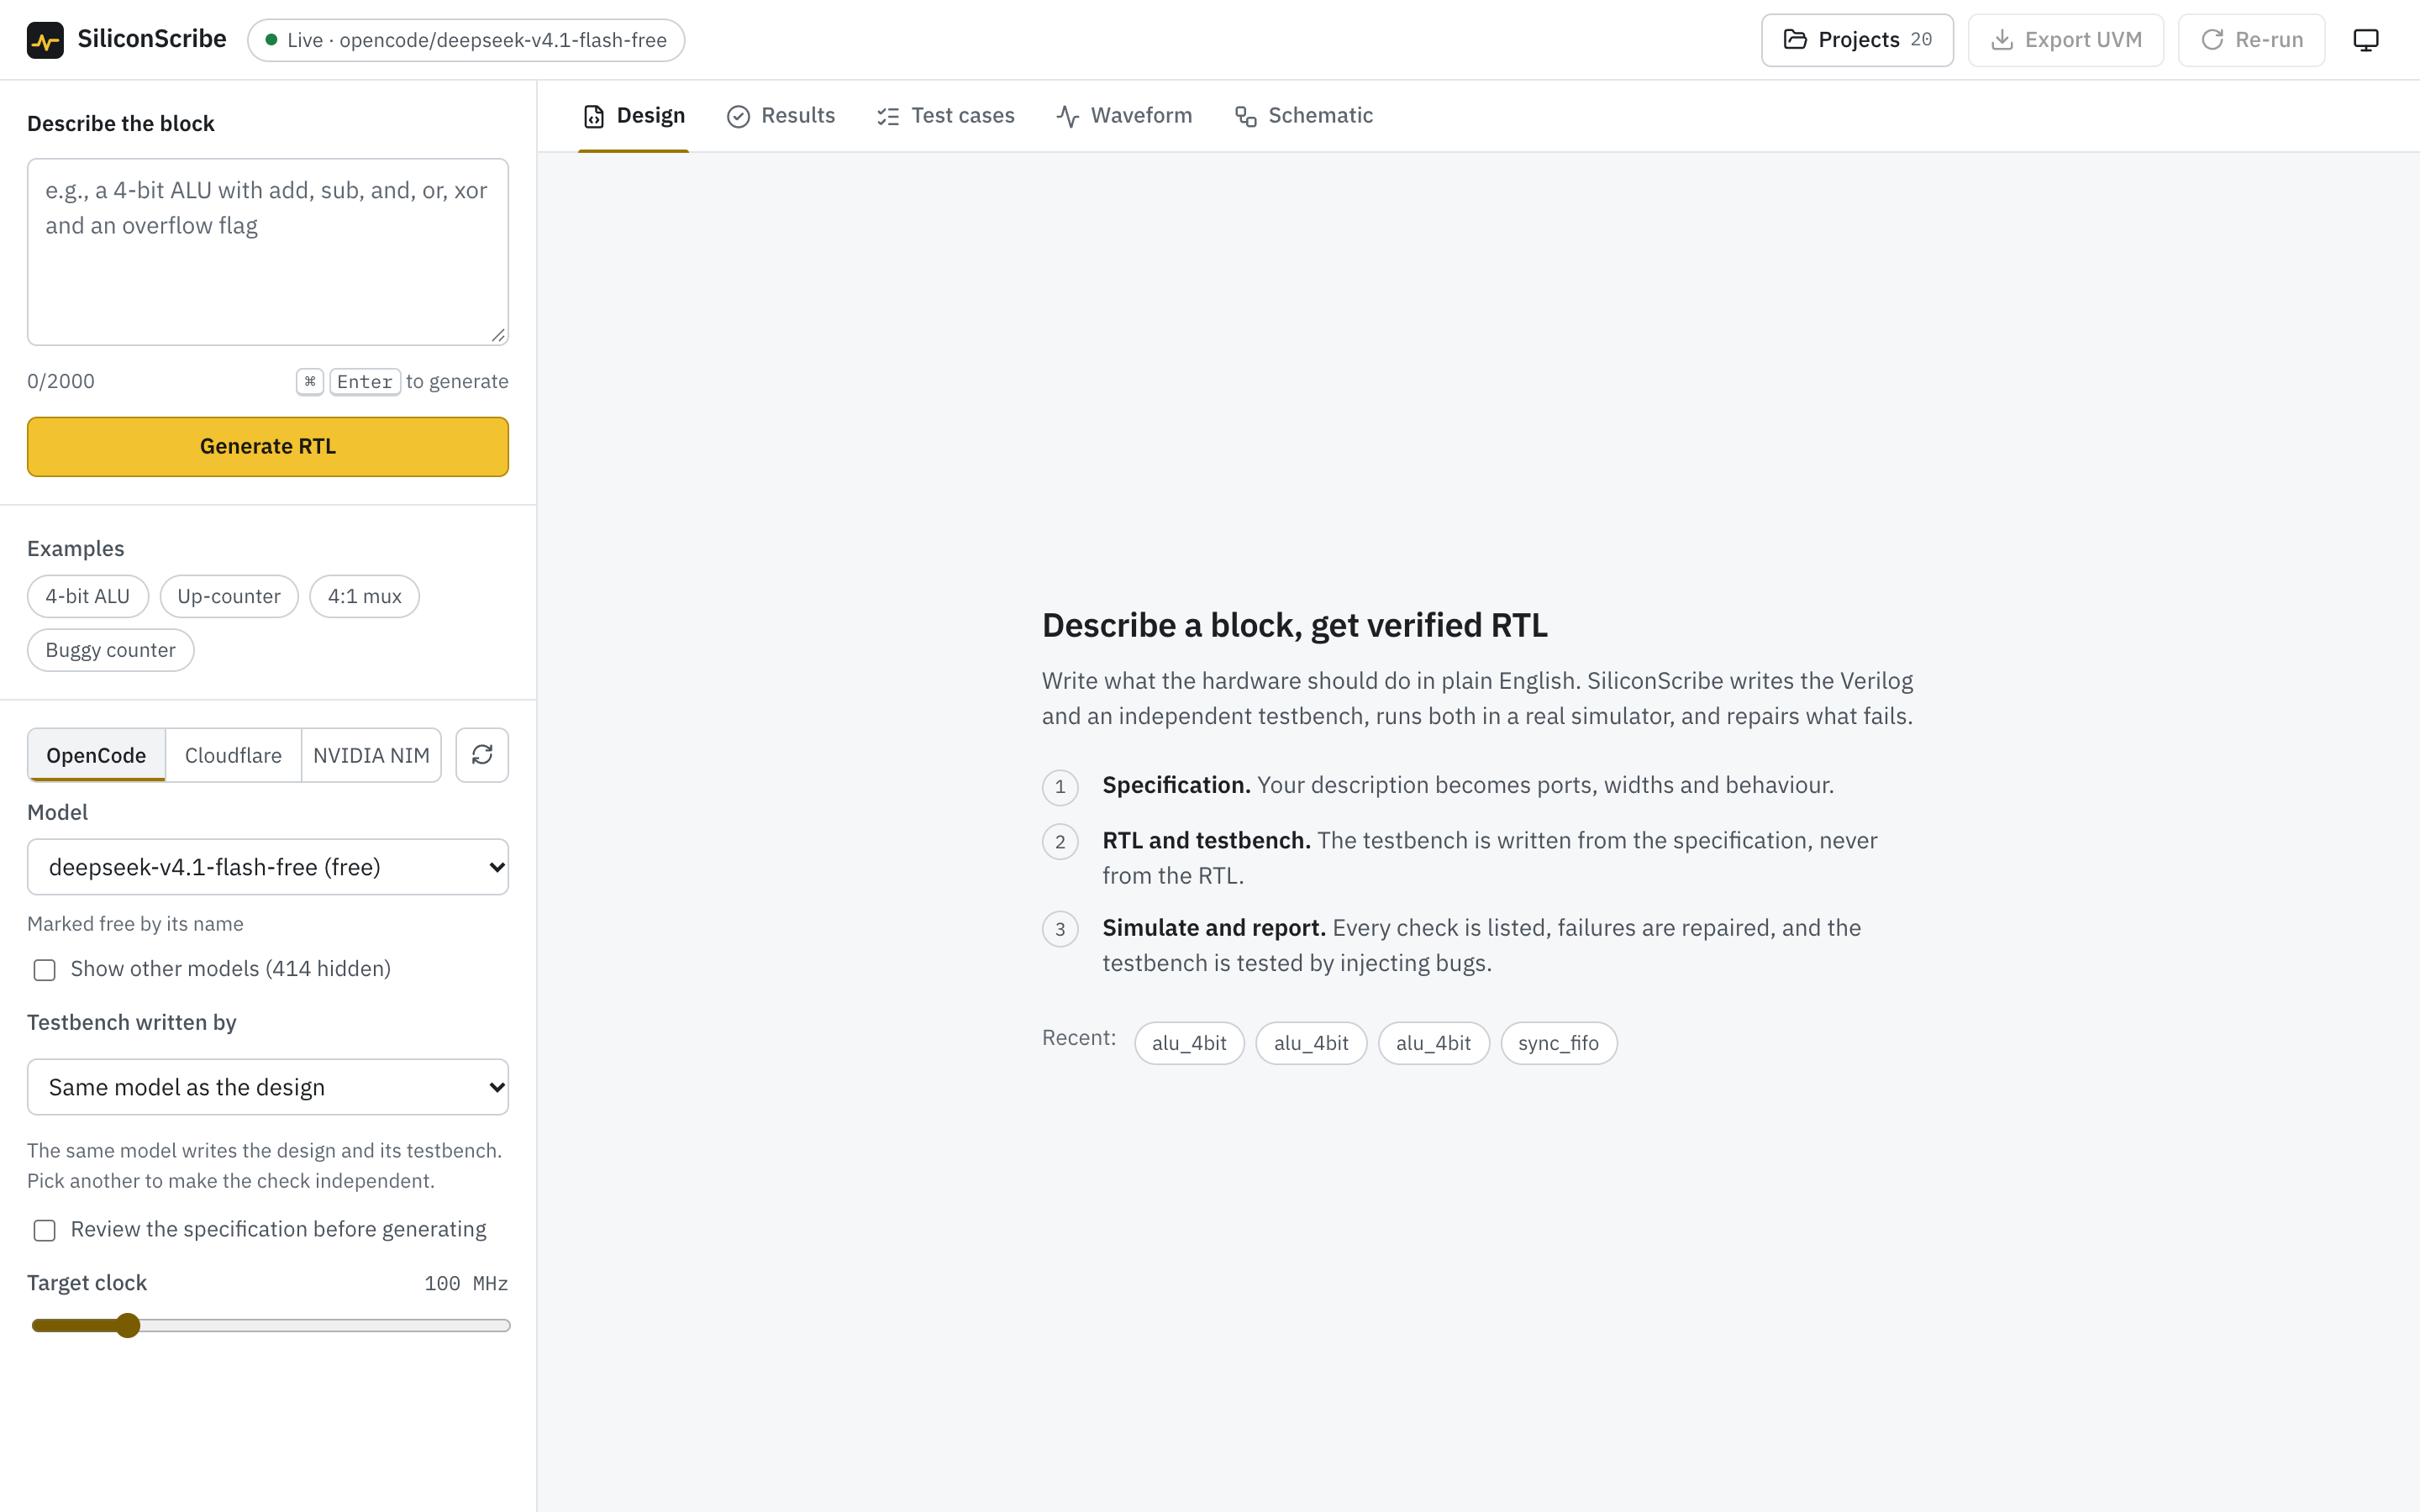
\includegraphics[width=0.92\textwidth]{s01_welcome.png}
\caption{Start screen of SiliconScribe. Before the first run, the Design tab explains the three steps and offers recent projects.}
\end{figure}

\section{The sidebar}

\begin{minipage}[t]{0.36\textwidth}
\vspace{0pt}
\centering
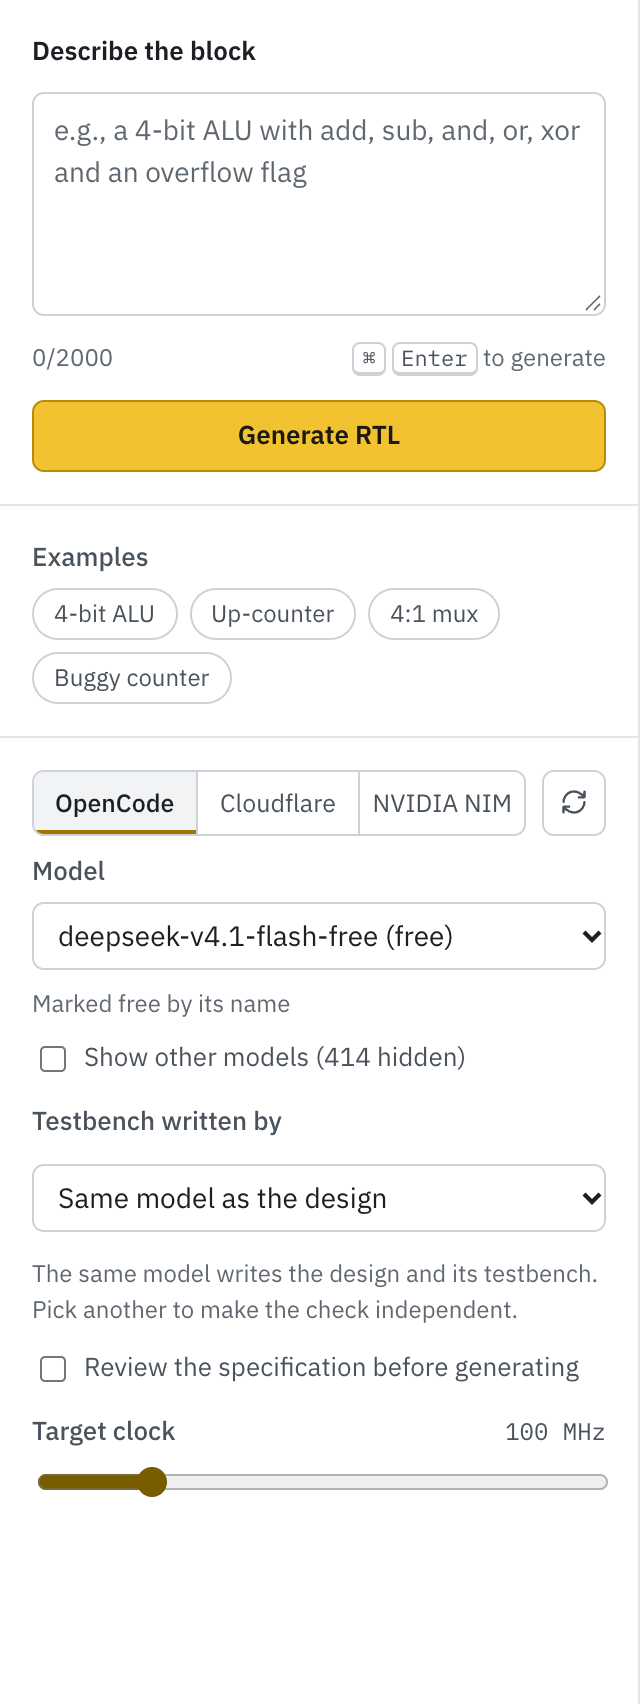
\includegraphics[height=0.52\textheight]{s02_model_menu.png}
\captionof{figure}{The sidebar with per-run model choice.}
\end{minipage}\hfill
\begin{minipage}[t]{0.6\textwidth}
\vspace{0pt}
From top to bottom:
\begin{description}
  \item[Describe the block] Up to 2000 characters, with a counter. Be specific about widths, reset style and behaviour. \textbf{Generate RTL} (or Ctrl/Cmd+Enter) starts the run.
  \item[Run] During and after a run, the run timeline appears right under the prompt (Section~\ref{sec:timeline}).
  \item[Examples] Four chips that fill the prompt: 4-bit ALU, Up-counter, 4:1 mux and Buggy counter (scripted only in offline mode).
  \item[Model menu] Three source tabs, \textbf{OpenCode}, \textbf{Cloudflare} and \textbf{NVIDIA NIM}, a refresh button, and the \textbf{Model} drop-down. Free models are marked ``(free)''; the note under the menu says why. On the OpenCode tab, \textbf{Show other models} lists the models not marked free (the number hidden is shown; they may use credits on your OpenCode account). Your choice is remembered in the browser.
  \item[Testbench written by] ``Same model as the design'' (default) or any other model from any tab. A separate model makes the check independent (Section~\ref{sec:independenttb}).
  \item[Review the specification before generating] When ticked, the run stops after the specification so you can check and edit it.
  \item[Target clock] 10 to 500 MHz (default 100). It is a hint for the RTL and the clock the timing estimate is checked against.
\end{description}
\end{minipage}

\section{Reviewing the specification}

With ``Review the specification before generating'' ticked, Generate RTL first asks the model only for the specification and shows it in the main pane: the module name, the ports (name, direction, width, description), any parameters, the \textbf{Behaviour} text and the \textbf{Constraints} (one per line). Correct anything that does not match what you meant, then press \textbf{Generate with this specification}; the run uses exactly that specification. \textbf{Cancel} goes back. This is not available in offline mode.

\begin{figure}[H]
\centering
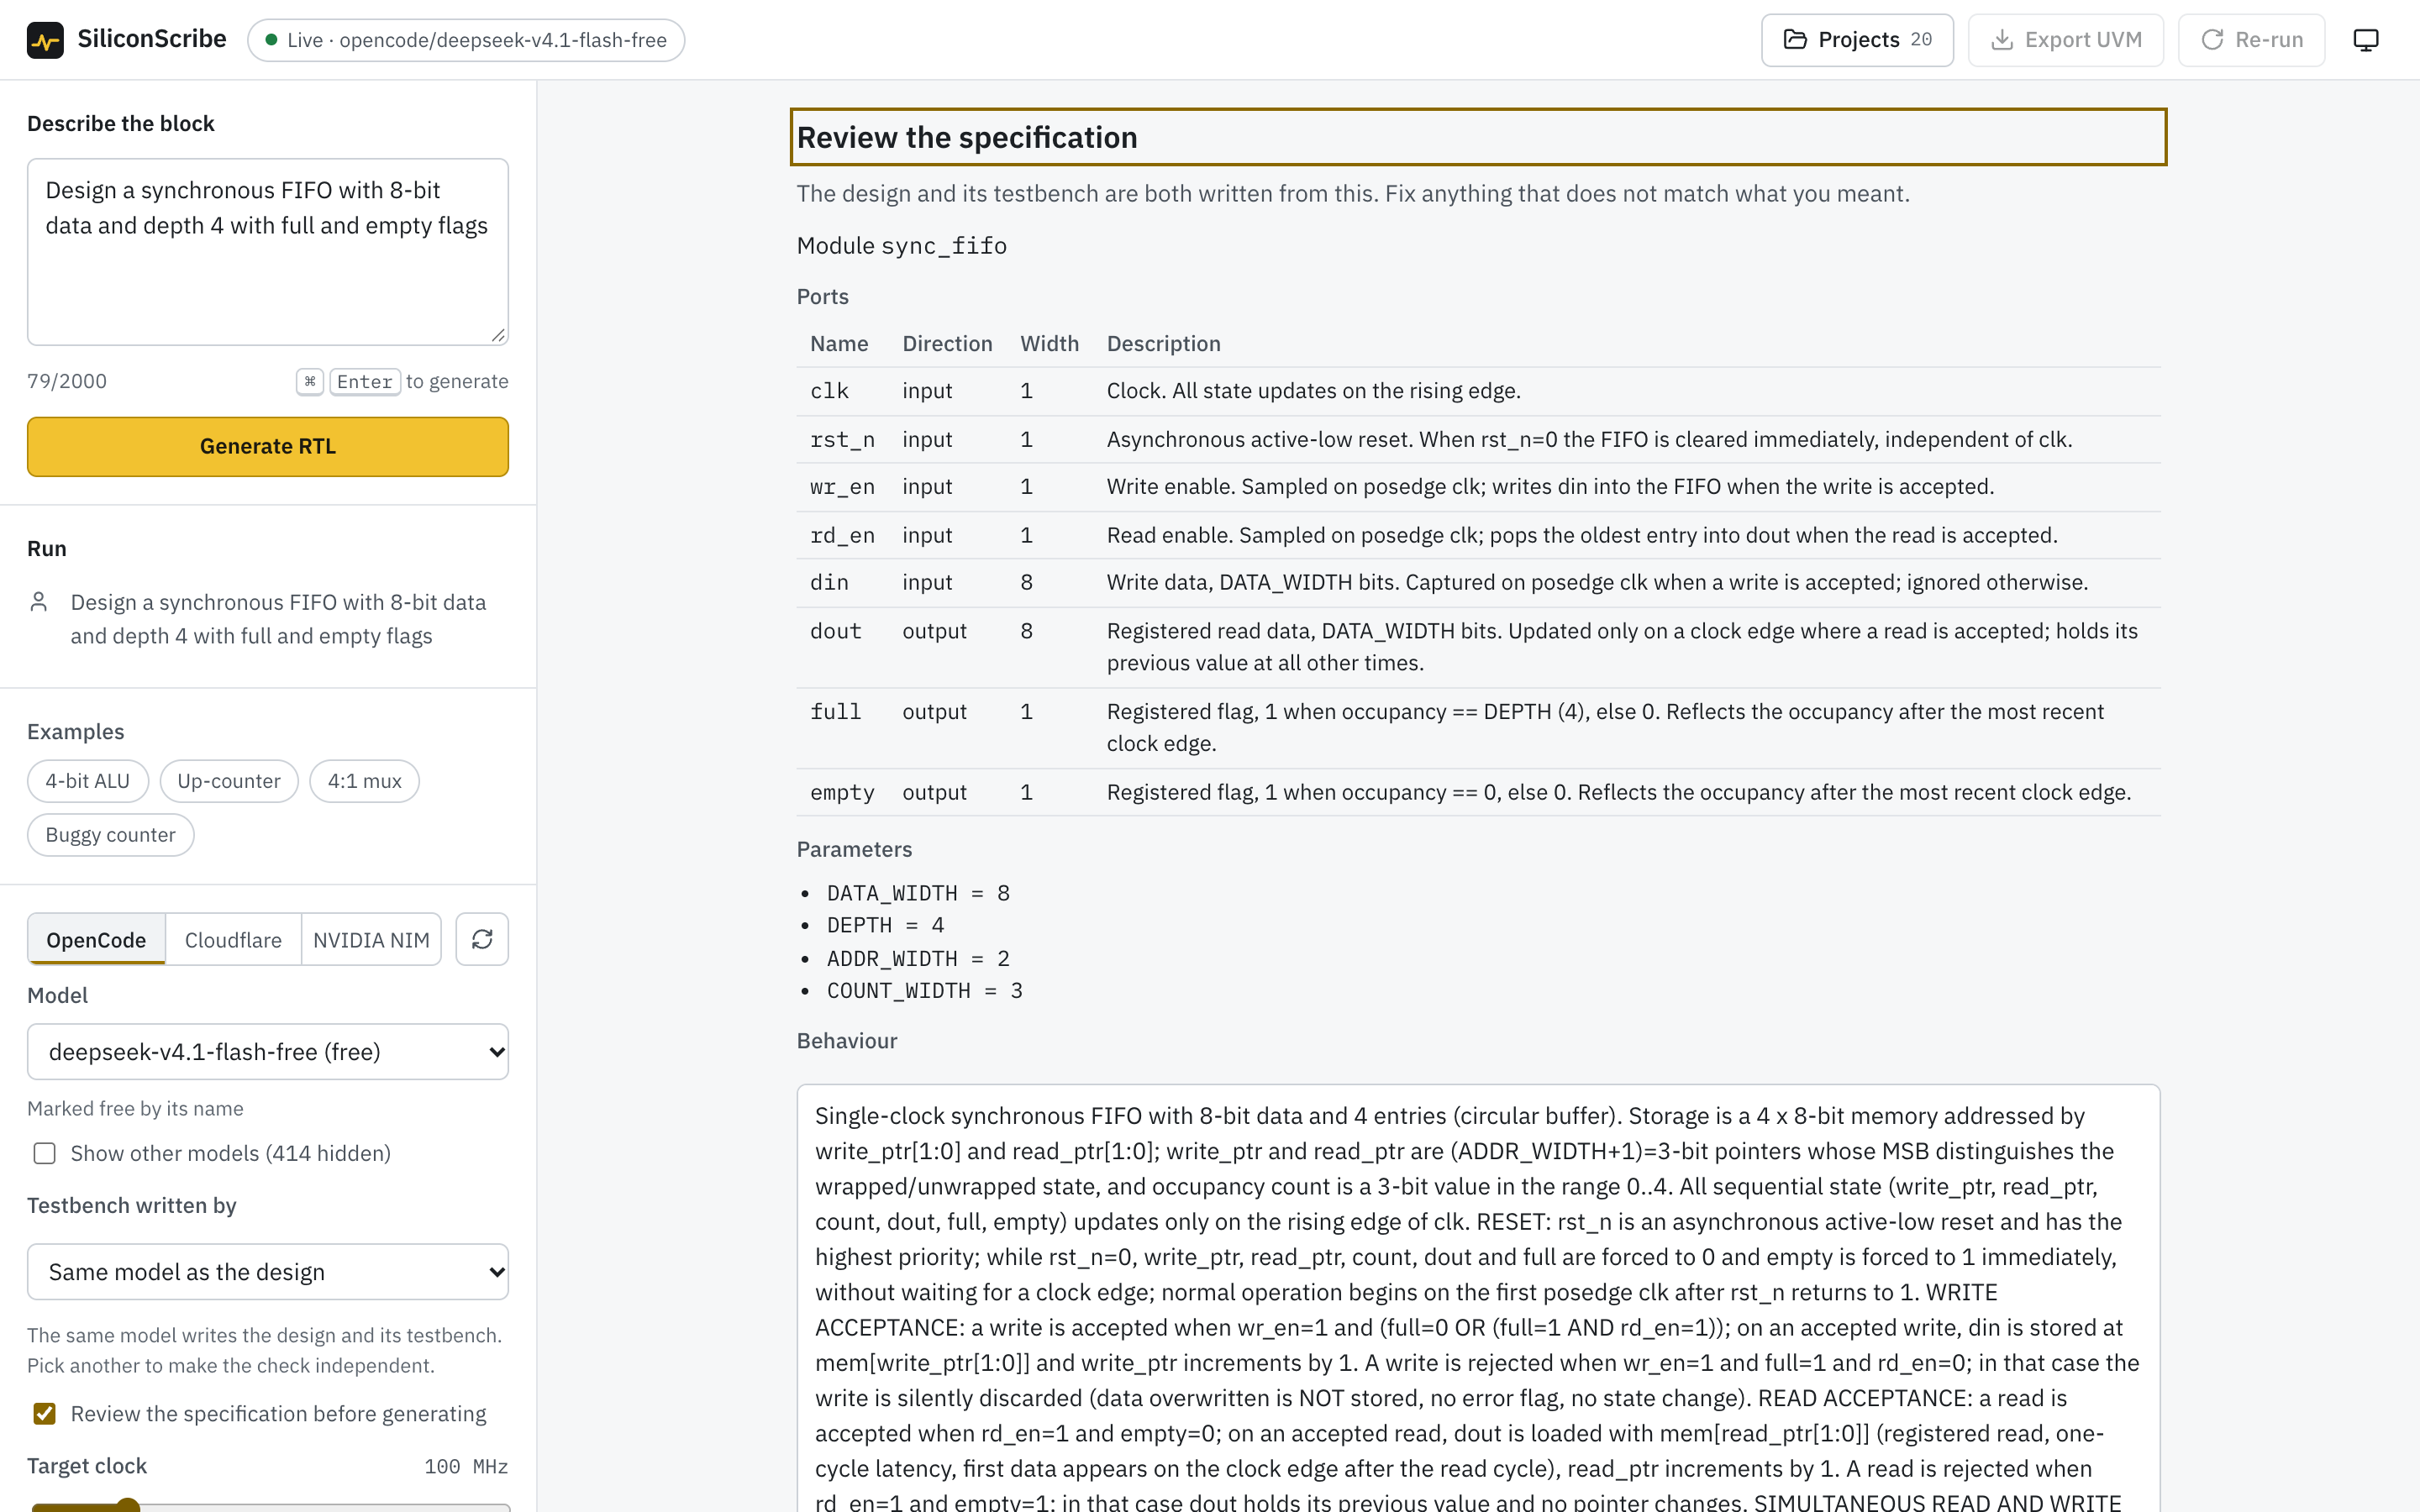
\includegraphics[width=0.92\textwidth]{s04_spec_review.png}
\caption{Reviewing the parsed specification before generation (a real specification written by the live model for a FIFO prompt).}
\end{figure}

\section{Watching the run}
\label{sec:timeline}

The run timeline lists one line per step: specification, RTL, lint, testbench, explanation, each simulation, each repair with its diagnosis (symptom, root cause, fix location, confidence), synthesis, the second opinion when there is one, testbench strength, timing, and the final message. While the run is going, a ``Working\ldots'' timer shows it is not stuck. Free models can take minutes per step. \textbf{Stop} in the top bar cancels the run.

\begin{figure}[H]
\centering
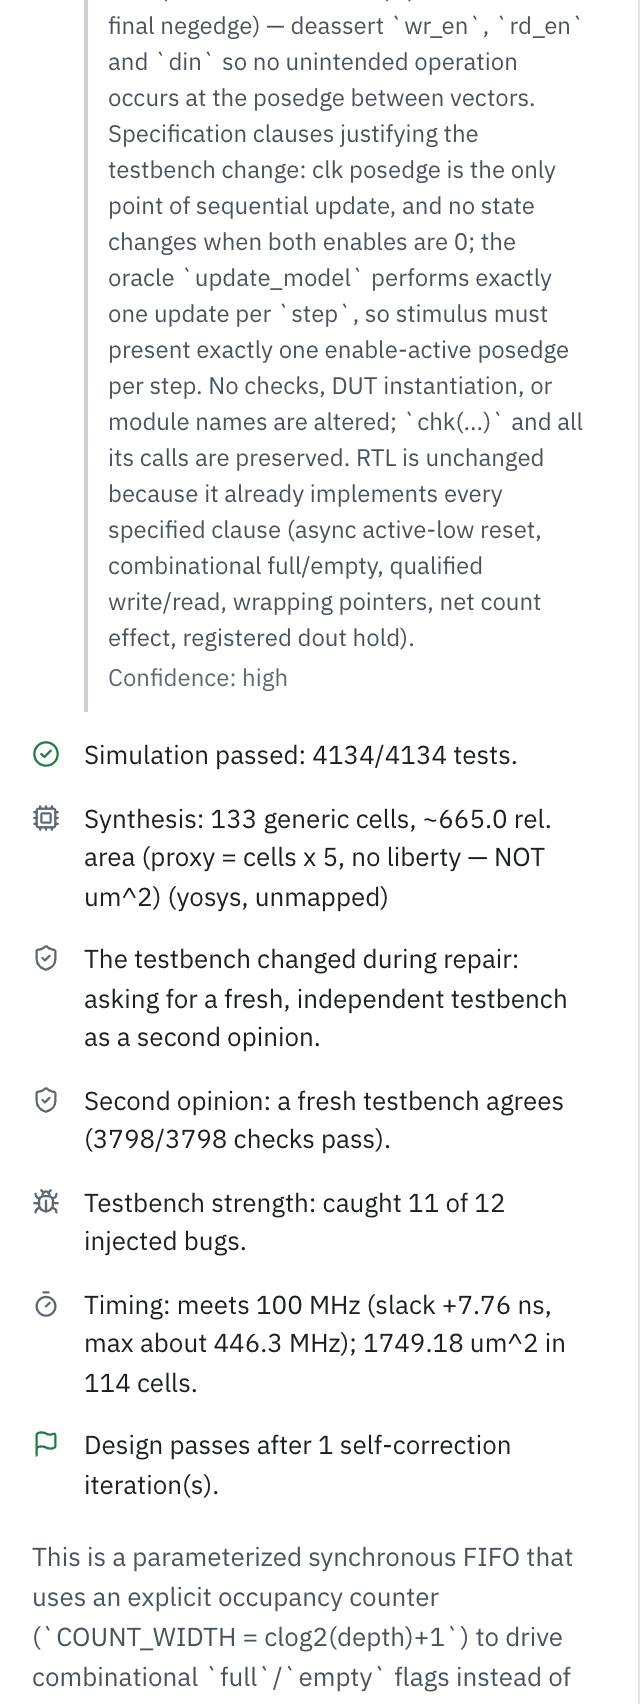
\includegraphics[height=0.5\textheight]{s05_run_timeline.png}
\caption{The run timeline of a real FIFO run (opencode/hy4-flash-free): one repair, then the second opinion, strength and timing steps.}
\end{figure}

\section{A first run, step by step}

\begin{enumerate}
  \item Click an example or type your own description.
  \item Choose a model (or keep the default), and optionally a separate testbench model, the specification review and a target clock.
  \item Press \textbf{Generate RTL}. The Design tab shows the code as it arrives; the timeline shows each step.
  \item When the run ends, the Results tab opens. Read the verdict first, then the sections below it.
  \item Open \textbf{Test cases} to see every check, \textbf{Waveform} to see the signals, \textbf{Schematic} for the block diagram.
  \item The run is saved automatically and appears in the \textbf{Projects} menu.
\end{enumerate}

\section{Reading the Results tab}

\begin{figure}[H]
\centering
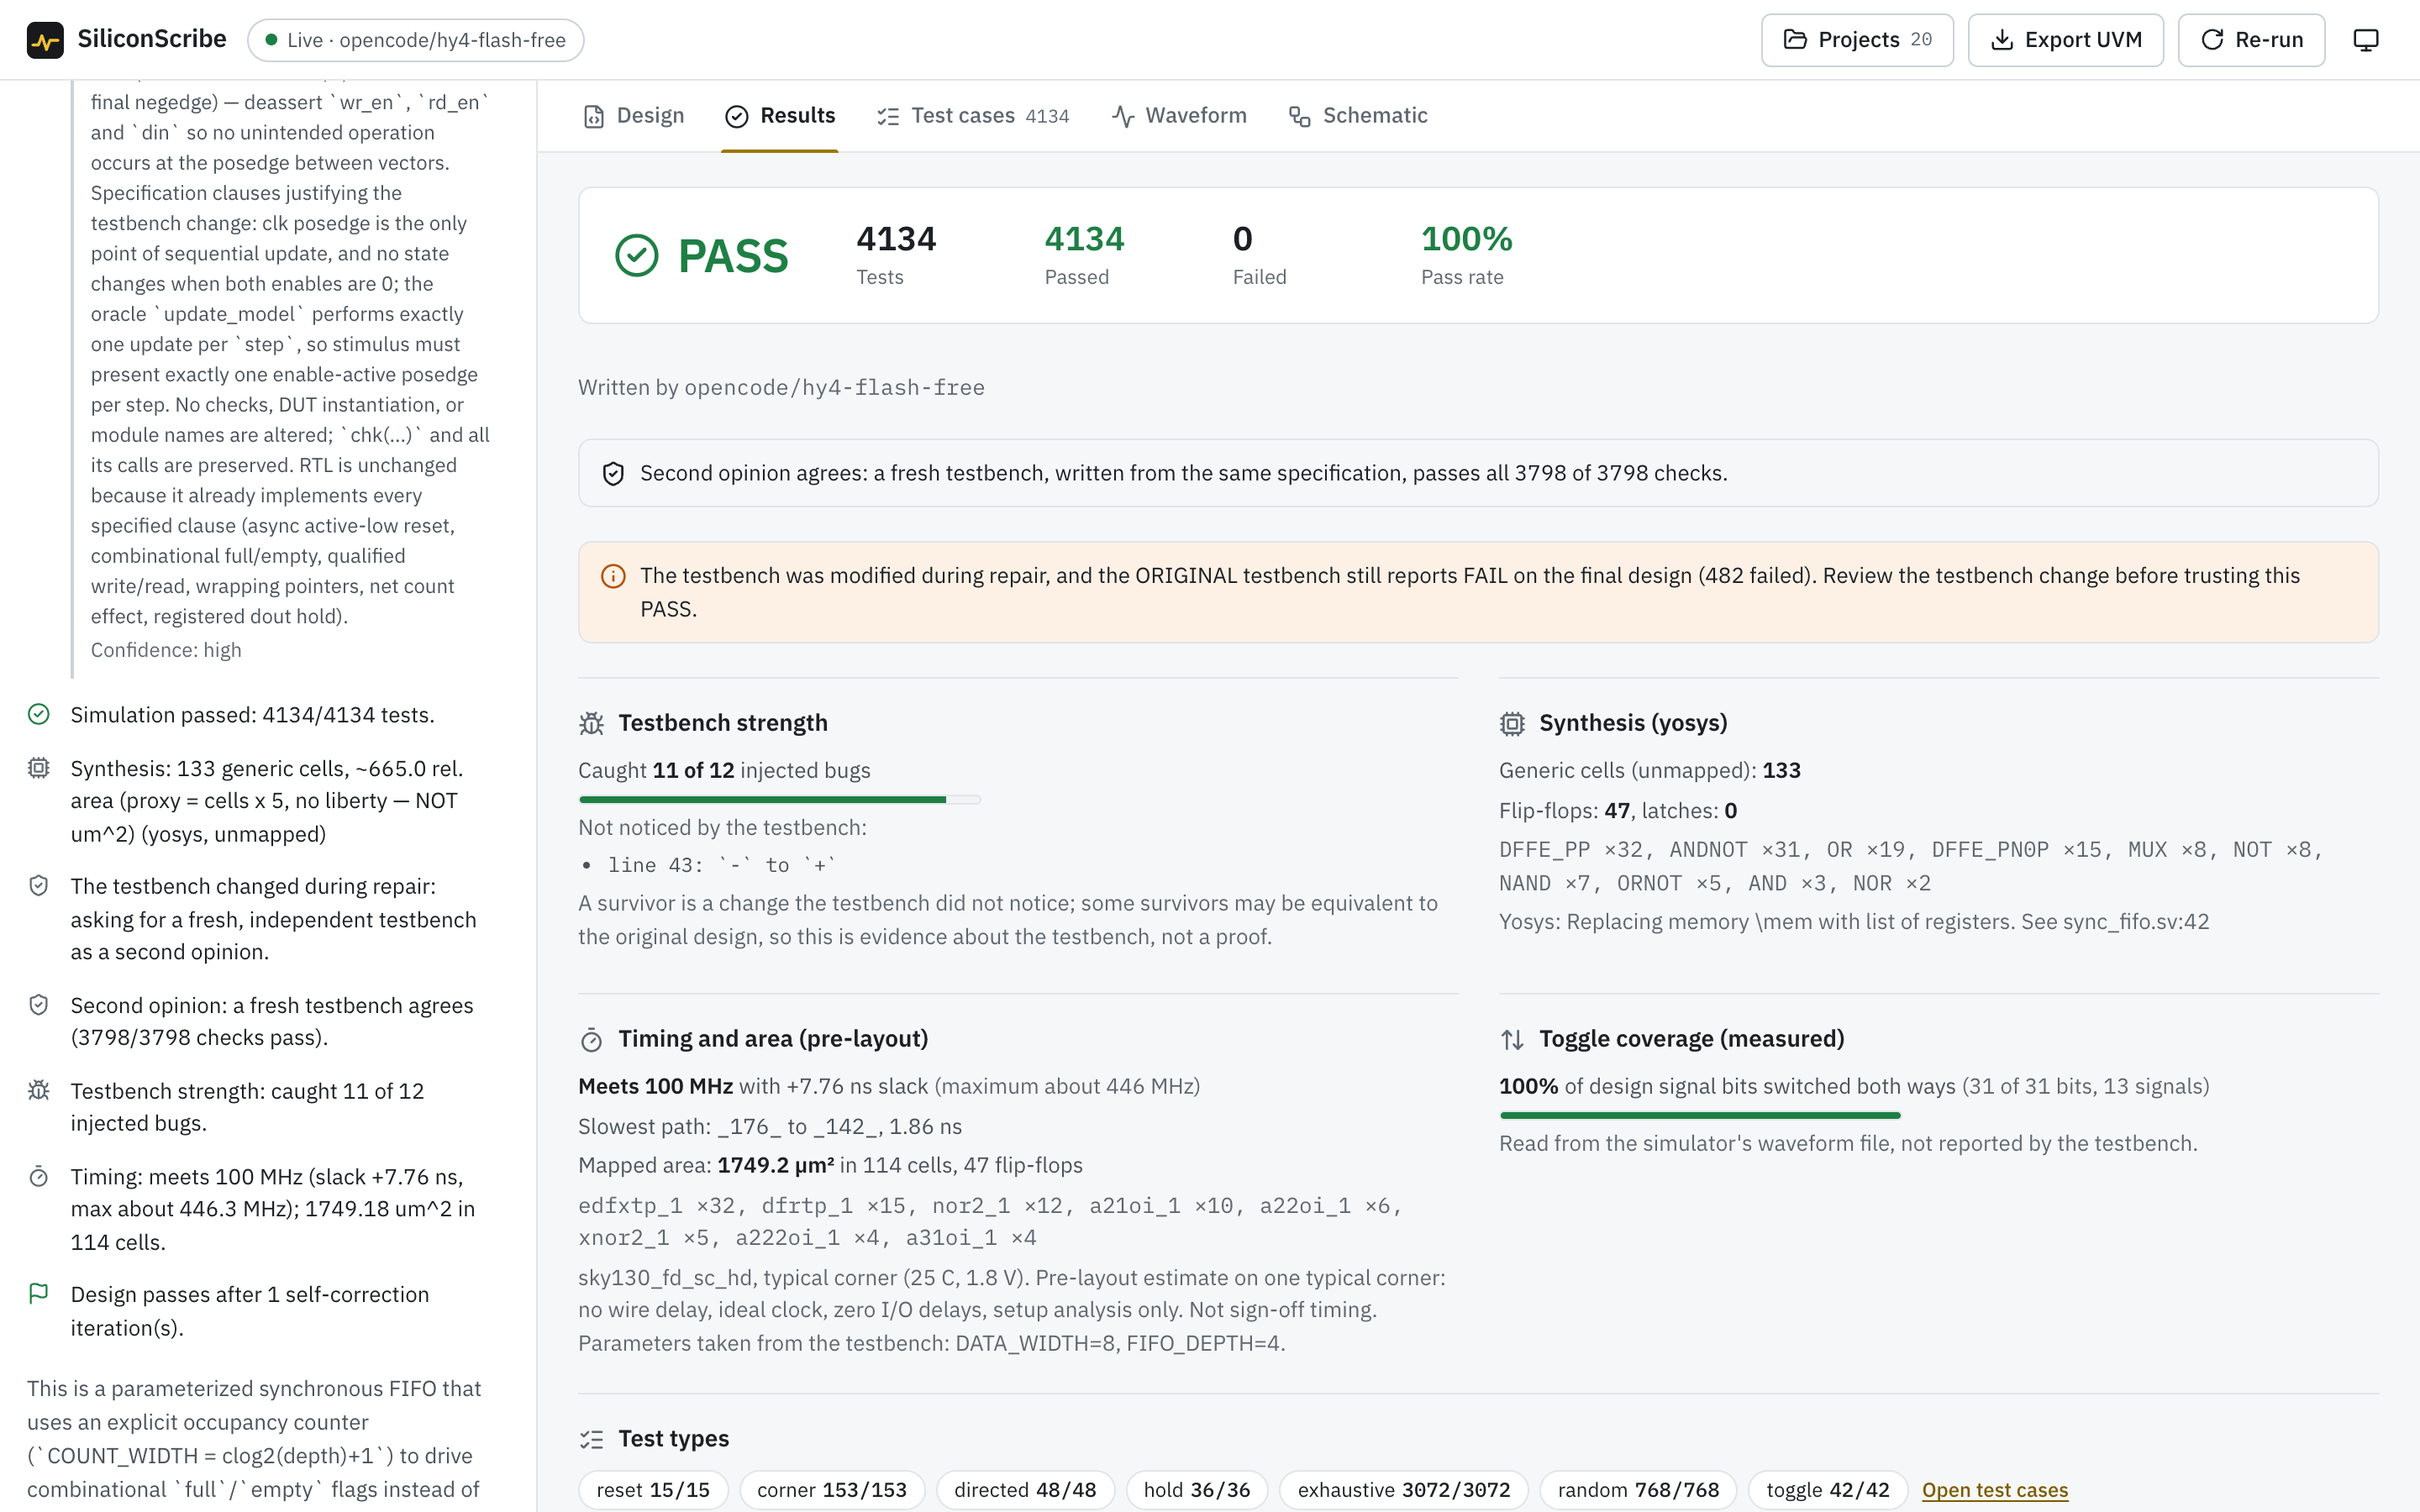
\includegraphics[width=0.95\textwidth]{s06_results_pass.png}
\caption{Results of a real FIFO run (opencode/hy4-flash-free): PASS 4134/4134 after one repair, the second opinion agrees (3798/3798), and a warning that the original testbench still fails on the final design (482 failed). Strength 11 of 12, timing meets 100 MHz, toggle coverage 100\%.}
\end{figure}

\begin{description}
  \item[Verdict] The status badge and four numbers: Tests, Passed, Failed, Pass rate. PASS (the design ran and every check passed), FAIL (some checks failed), ERROR (compile or runtime problem, no valid summary, or zero checks), TIMEOUT (the simulation ran too long). These come from the simulator transcript, never from the model.
  \item[Written by] The model that wrote the design, and, if a separate model wrote the testbench, ``Testbench written by \ldots, a separate model''. It is not shown for an offline result or after a Re-run of edited code.
  \item[Second opinion] Shown only when a repair rewrote the testbench: agrees, disagrees (do not trust this PASS) or not obtained, with the reason.
  \item[Warnings] Amber notes such as too few checks, a weak testbench, the original testbench still failing, or two models disagreeing. A grey ``Built-in demo result: not generated by the AI model for your prompt'' note marks a demo fallback.
  \item[Testbench strength] ``Caught N of M injected bugs'' with a bar, and the bugs that were not noticed (line and change). The bar turns amber when fewer than half were caught. A survivor may be an equivalent change (Section~\ref{sec:strength}).
  \item[Synthesis (yosys)] Generic (unmapped) cell count, flip-flops and latches, cell types, and any Yosys warning (with file names only, never the server's folder paths). The relative area proxy appears only when there is no mapped area.
  \item[Timing and area (pre-layout)] ``Meets'' or ``Misses'' the target clock with the slack and the maximum frequency; for a design with no clock, ``Longest input-to-output path'' instead. Then the slowest path, the mapped area in \umsq{} with cell and flip-flop counts, the most common cells, and the limits line (one corner, no wire delay, ideal clock, setup only, not sign-off). If the estimate refused the design, the reason is shown instead of a number.
  \item[Toggle coverage (measured)] The percentage of design signal bits that switched both ways, with counts and the signals that never switched. It is read from the simulator's waveform file.
  \item[Test types] One chip per type of check (for example reset, corner, directed, hold, random), with ``Open test cases''.
  \item[Lint, Self-correction loop, Errors] Lint findings; each repair attempt with its status, counts and fix type (\emph{compiler\_repair} and \emph{llm\_diagnosis} are real fixes; \emph{offline\_scripted} is the labelled demo path with no invented root cause); the error lines of a failed run.
  \item[Specification the design was built from] A fold-out, read-only copy of the specification that was used.
\end{description}

\begin{figure}[H]
\centering
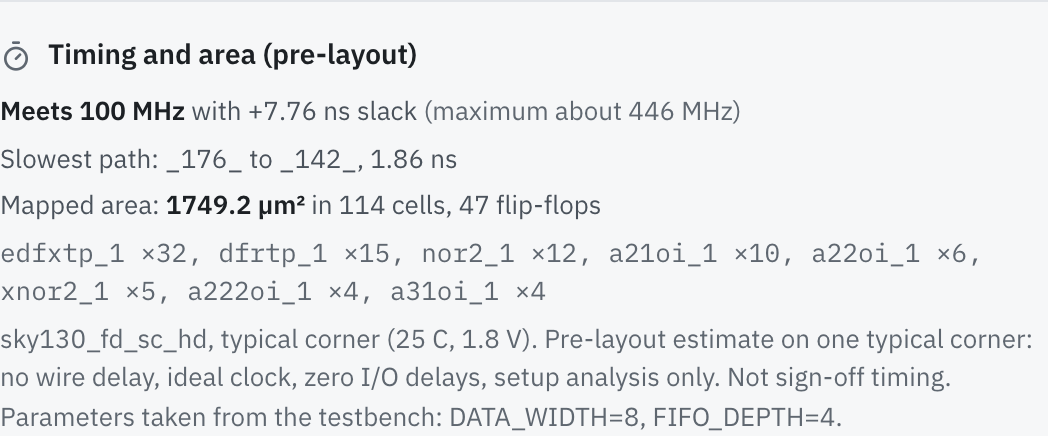
\includegraphics[width=0.62\textwidth]{s07_timing_section.png}
\caption{The ``Timing and area (pre-layout)'' section with its limits line.}
\end{figure}

\begin{figure}[H]
\centering
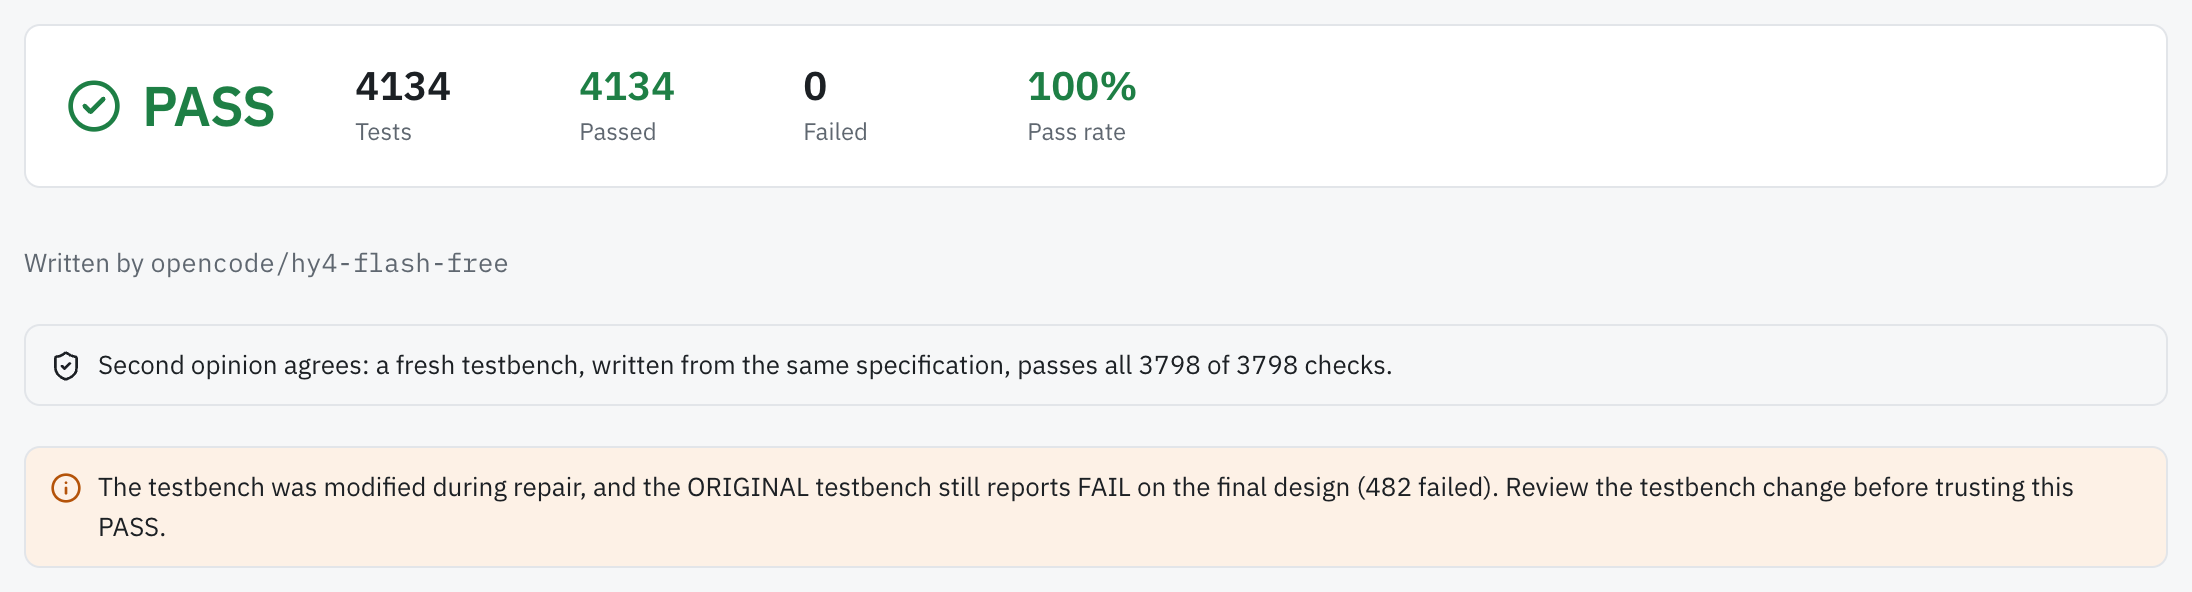
\includegraphics[width=0.92\textwidth]{s08_second_opinion.png}
\caption{The second opinion and the testbench-change warning are both shown.}
\end{figure}

\section{The Test cases tab}
\label{sec:testcases}

The Results tab only says ``4134 passed''. The Test cases tab shows \emph{which} checks ran. At the top, a bar and the totals; below it one chip per test type showing how many of that type passed; click a chip to filter. The table lists each check's number, type, name, simulation time, expected value, actual value and result. Use the Failed filter to see only failures, search by name, or click a row to see a bit-by-bit comparison with the differing bits highlighted and a \textbf{Show in waveform} button that jumps to that moment. Long runs stay fast because only the visible rows are drawn, and a note says when the list is capped (the totals are always exact). Testbenches that do not use the standard \texttt{chk} task show only totals, and the tab says so rather than inventing a list.

\begin{figure}[H]
\centering
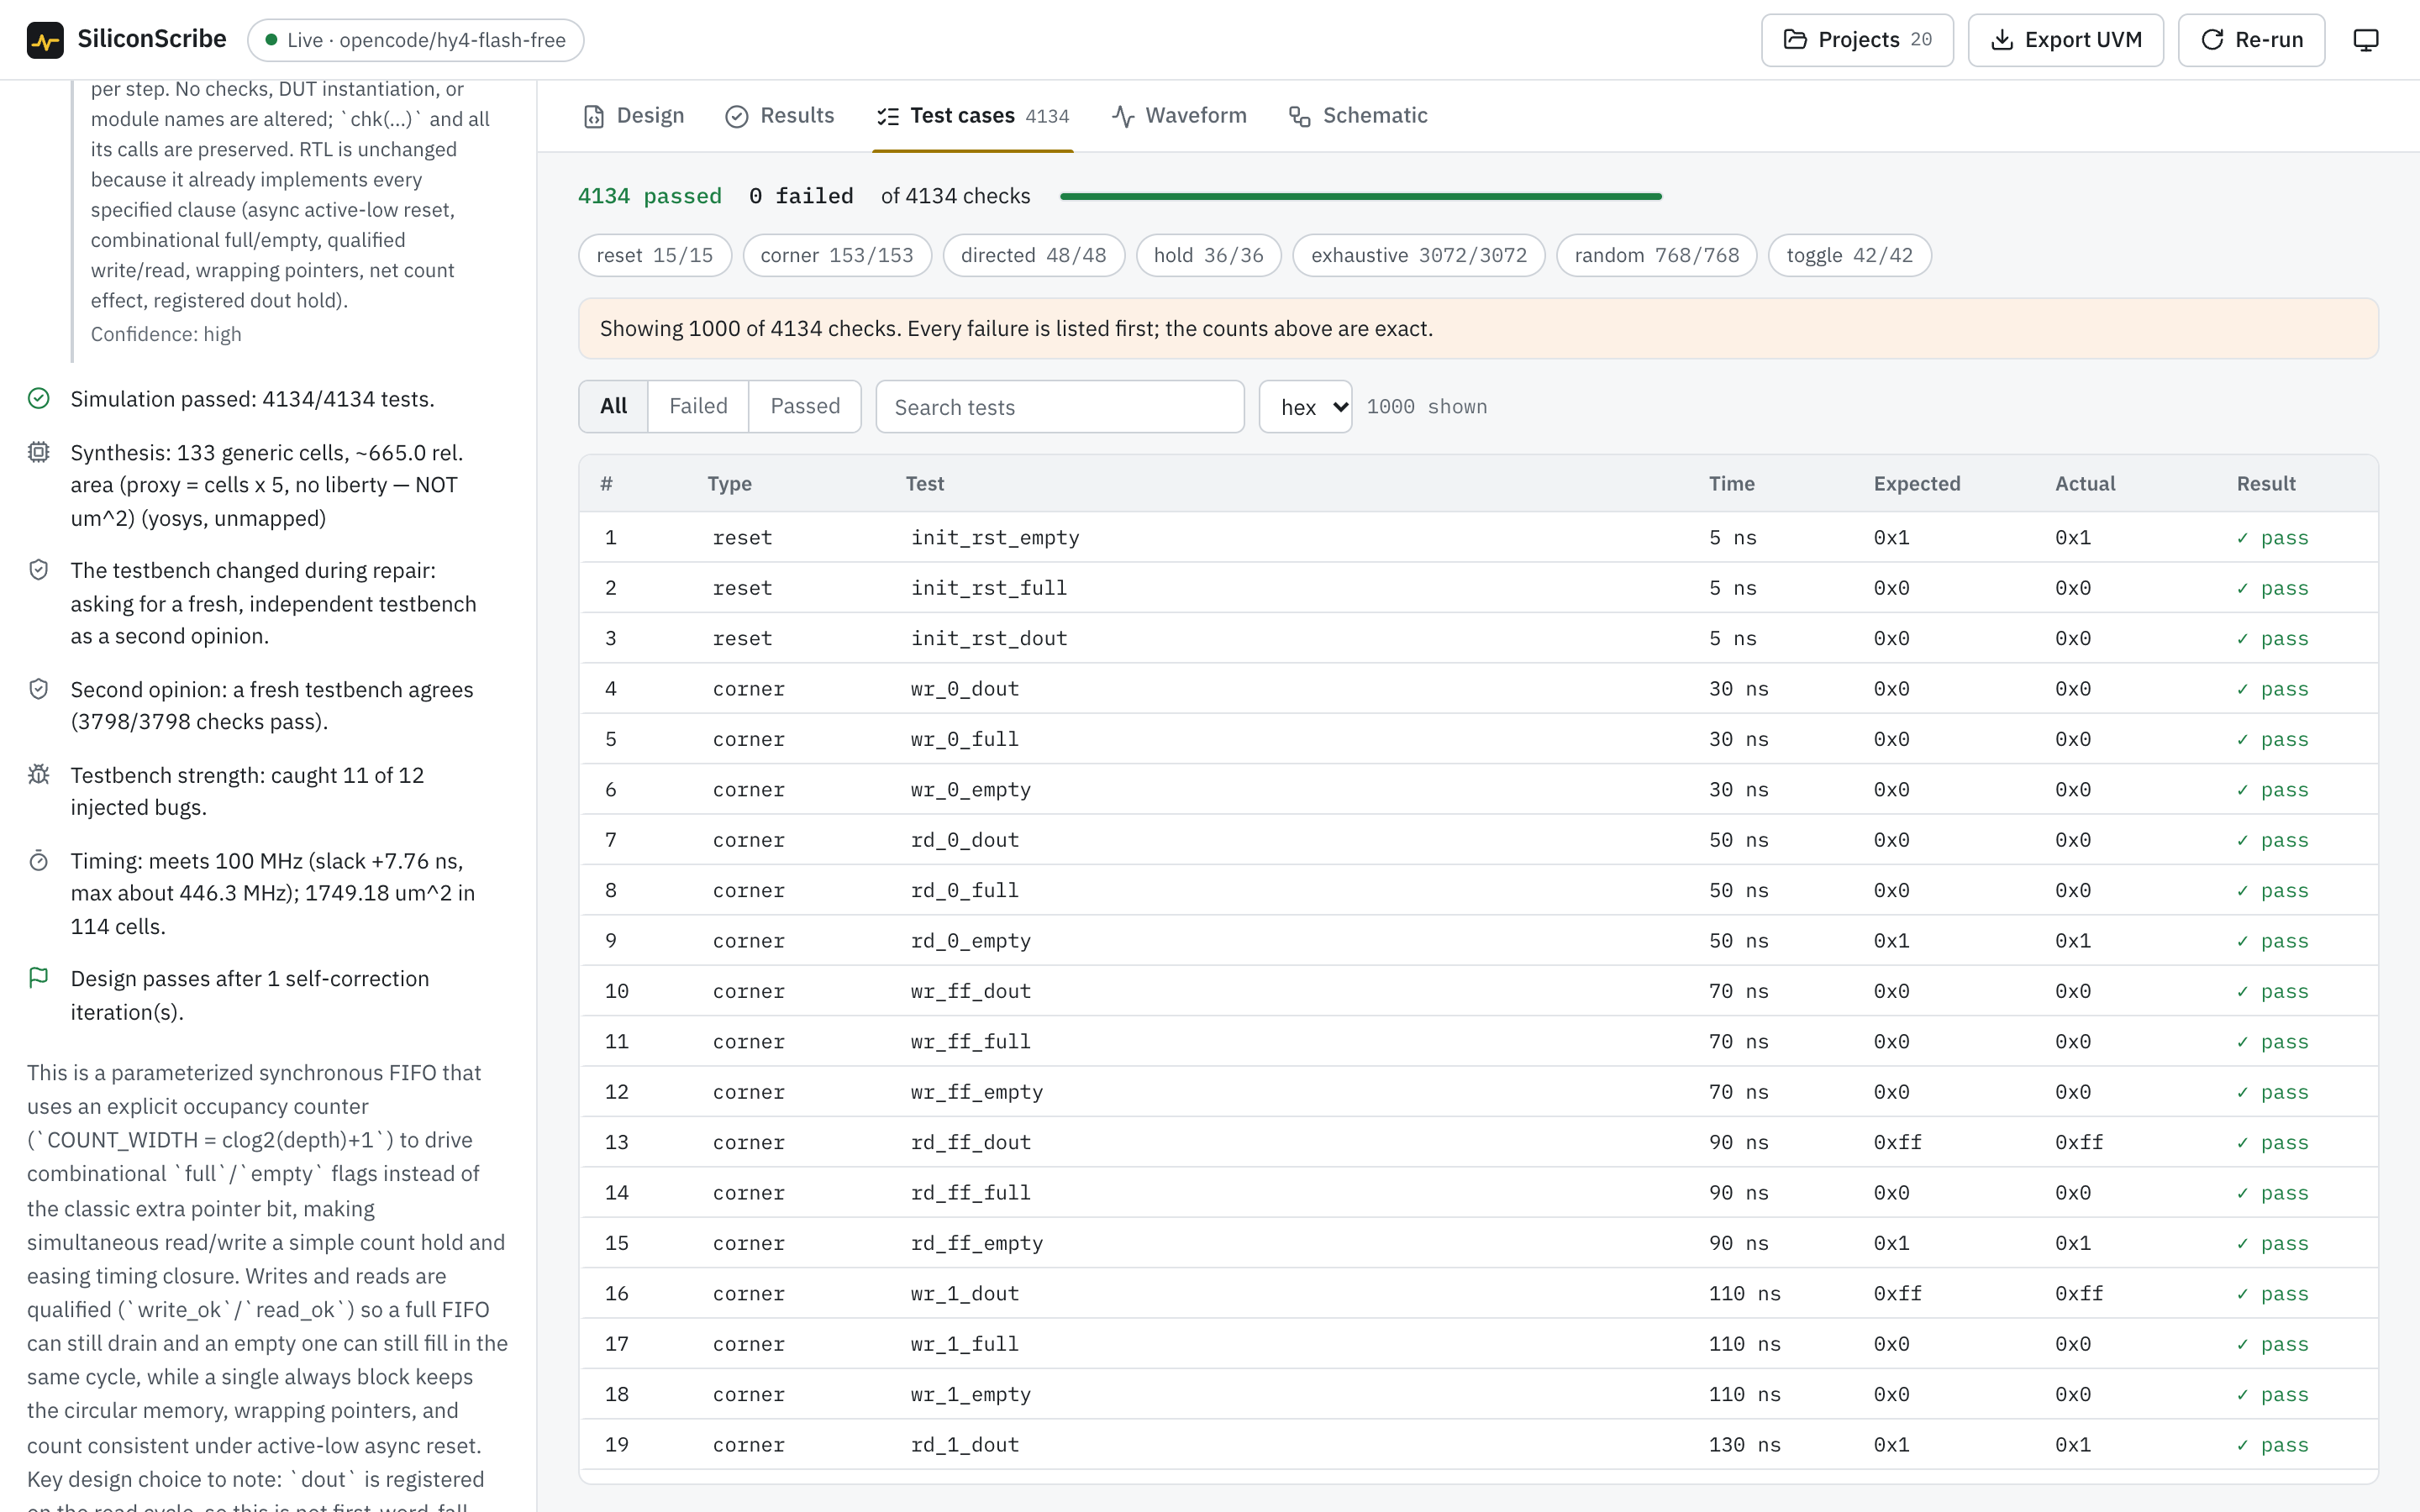
\includegraphics[width=0.92\textwidth]{s09_test_cases.png}
\caption{The Test cases tab of the FIFO run: 4134 checks grouped by type.}
\end{figure}

\section{The Waveform tab}

The waveform opens fitted to the pane. Signals are grouped by role (clock and reset, inputs, outputs, internal); the testbench's own variables are hidden until you ask for them. Click the plot to place cursor A, Shift+click for cursor B (the readout shows the time difference), and the signal-name column shows every signal's value at the cursor in hex, binary or decimal. Red flags on the time axis mark failed checks; press \texttt{]} and \texttt{[} to step between them. Use + and $-$ (or Ctrl/Cmd and the scroll wheel) to zoom and Reset to fit again, and \textbf{Expand} to give the whole results pane the full window (Esc restores it).

\begin{figure}[H]
\centering
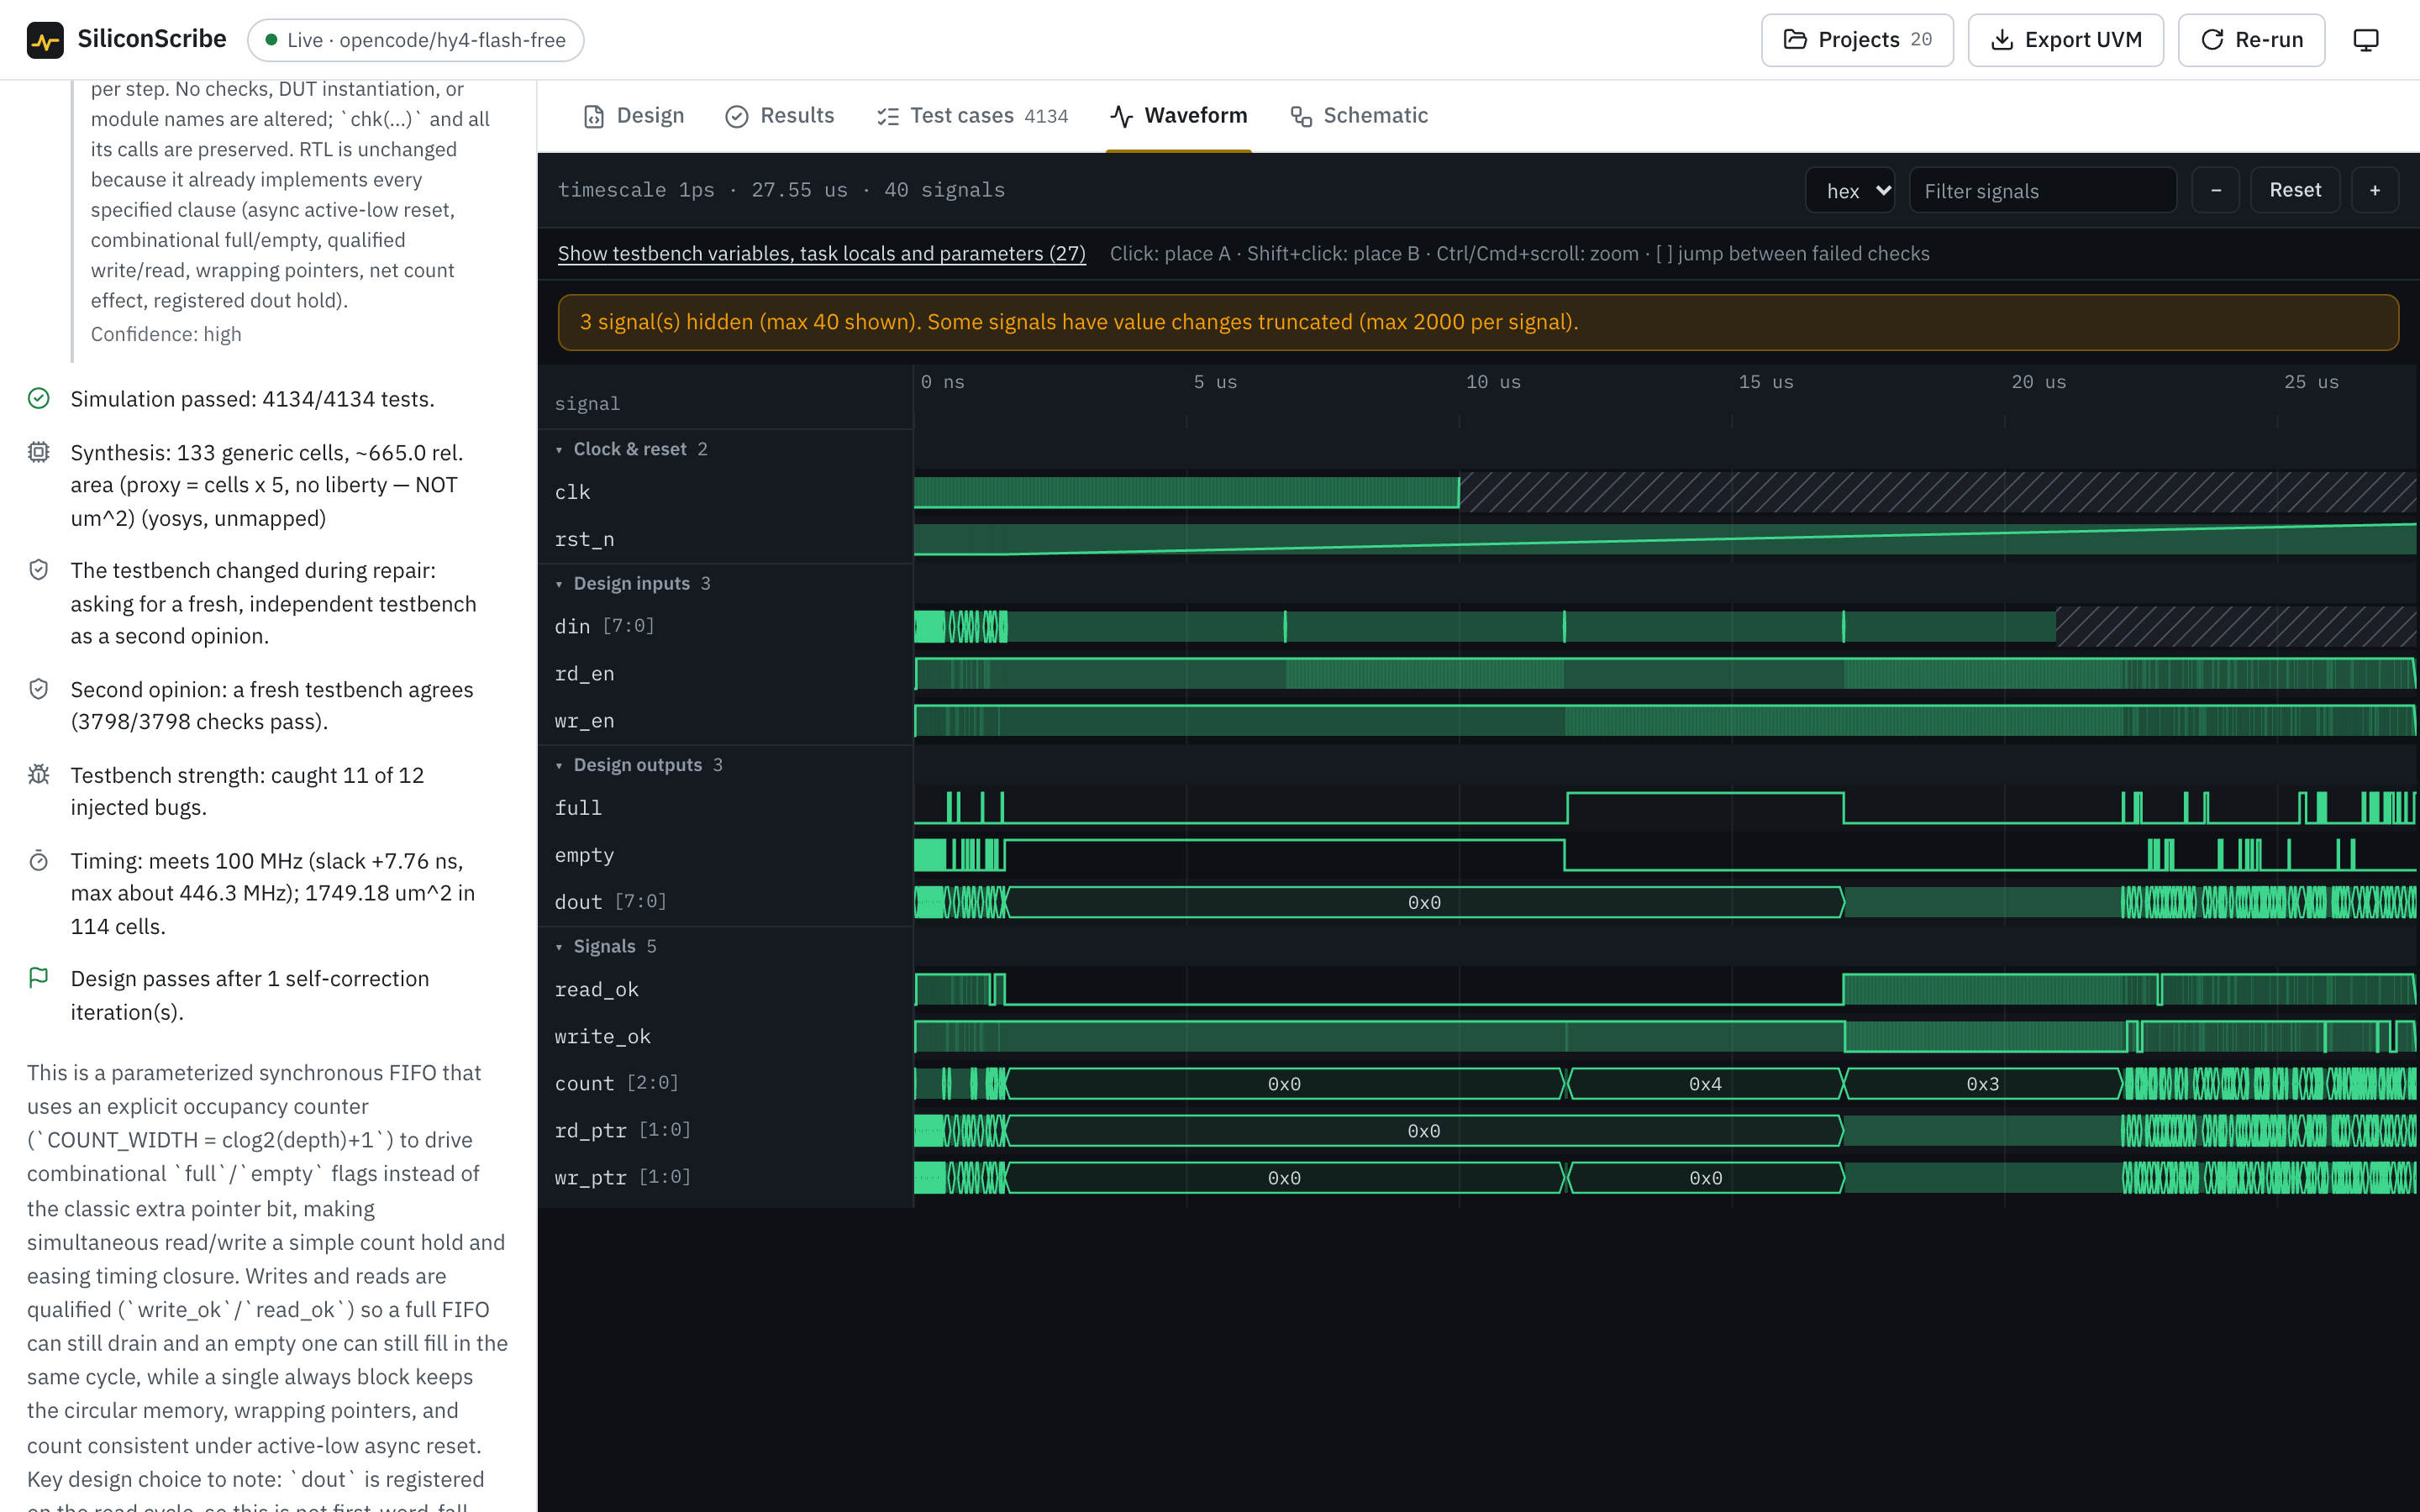
\includegraphics[width=0.92\textwidth]{s10_waveform.png}
\caption{The Waveform tab of the FIFO run.}
\end{figure}

\section{The Schematic and Design tabs}

The Schematic tab shows a port-level block diagram: the module as a box with inputs on the left, outputs on the right and widths such as \code{[7:0]}. A gate-level view of the synthesized netlist is not drawn; the tab says it is future work. The Design tab holds the RTL and testbench editors.

\begin{figure}[H]
\centering
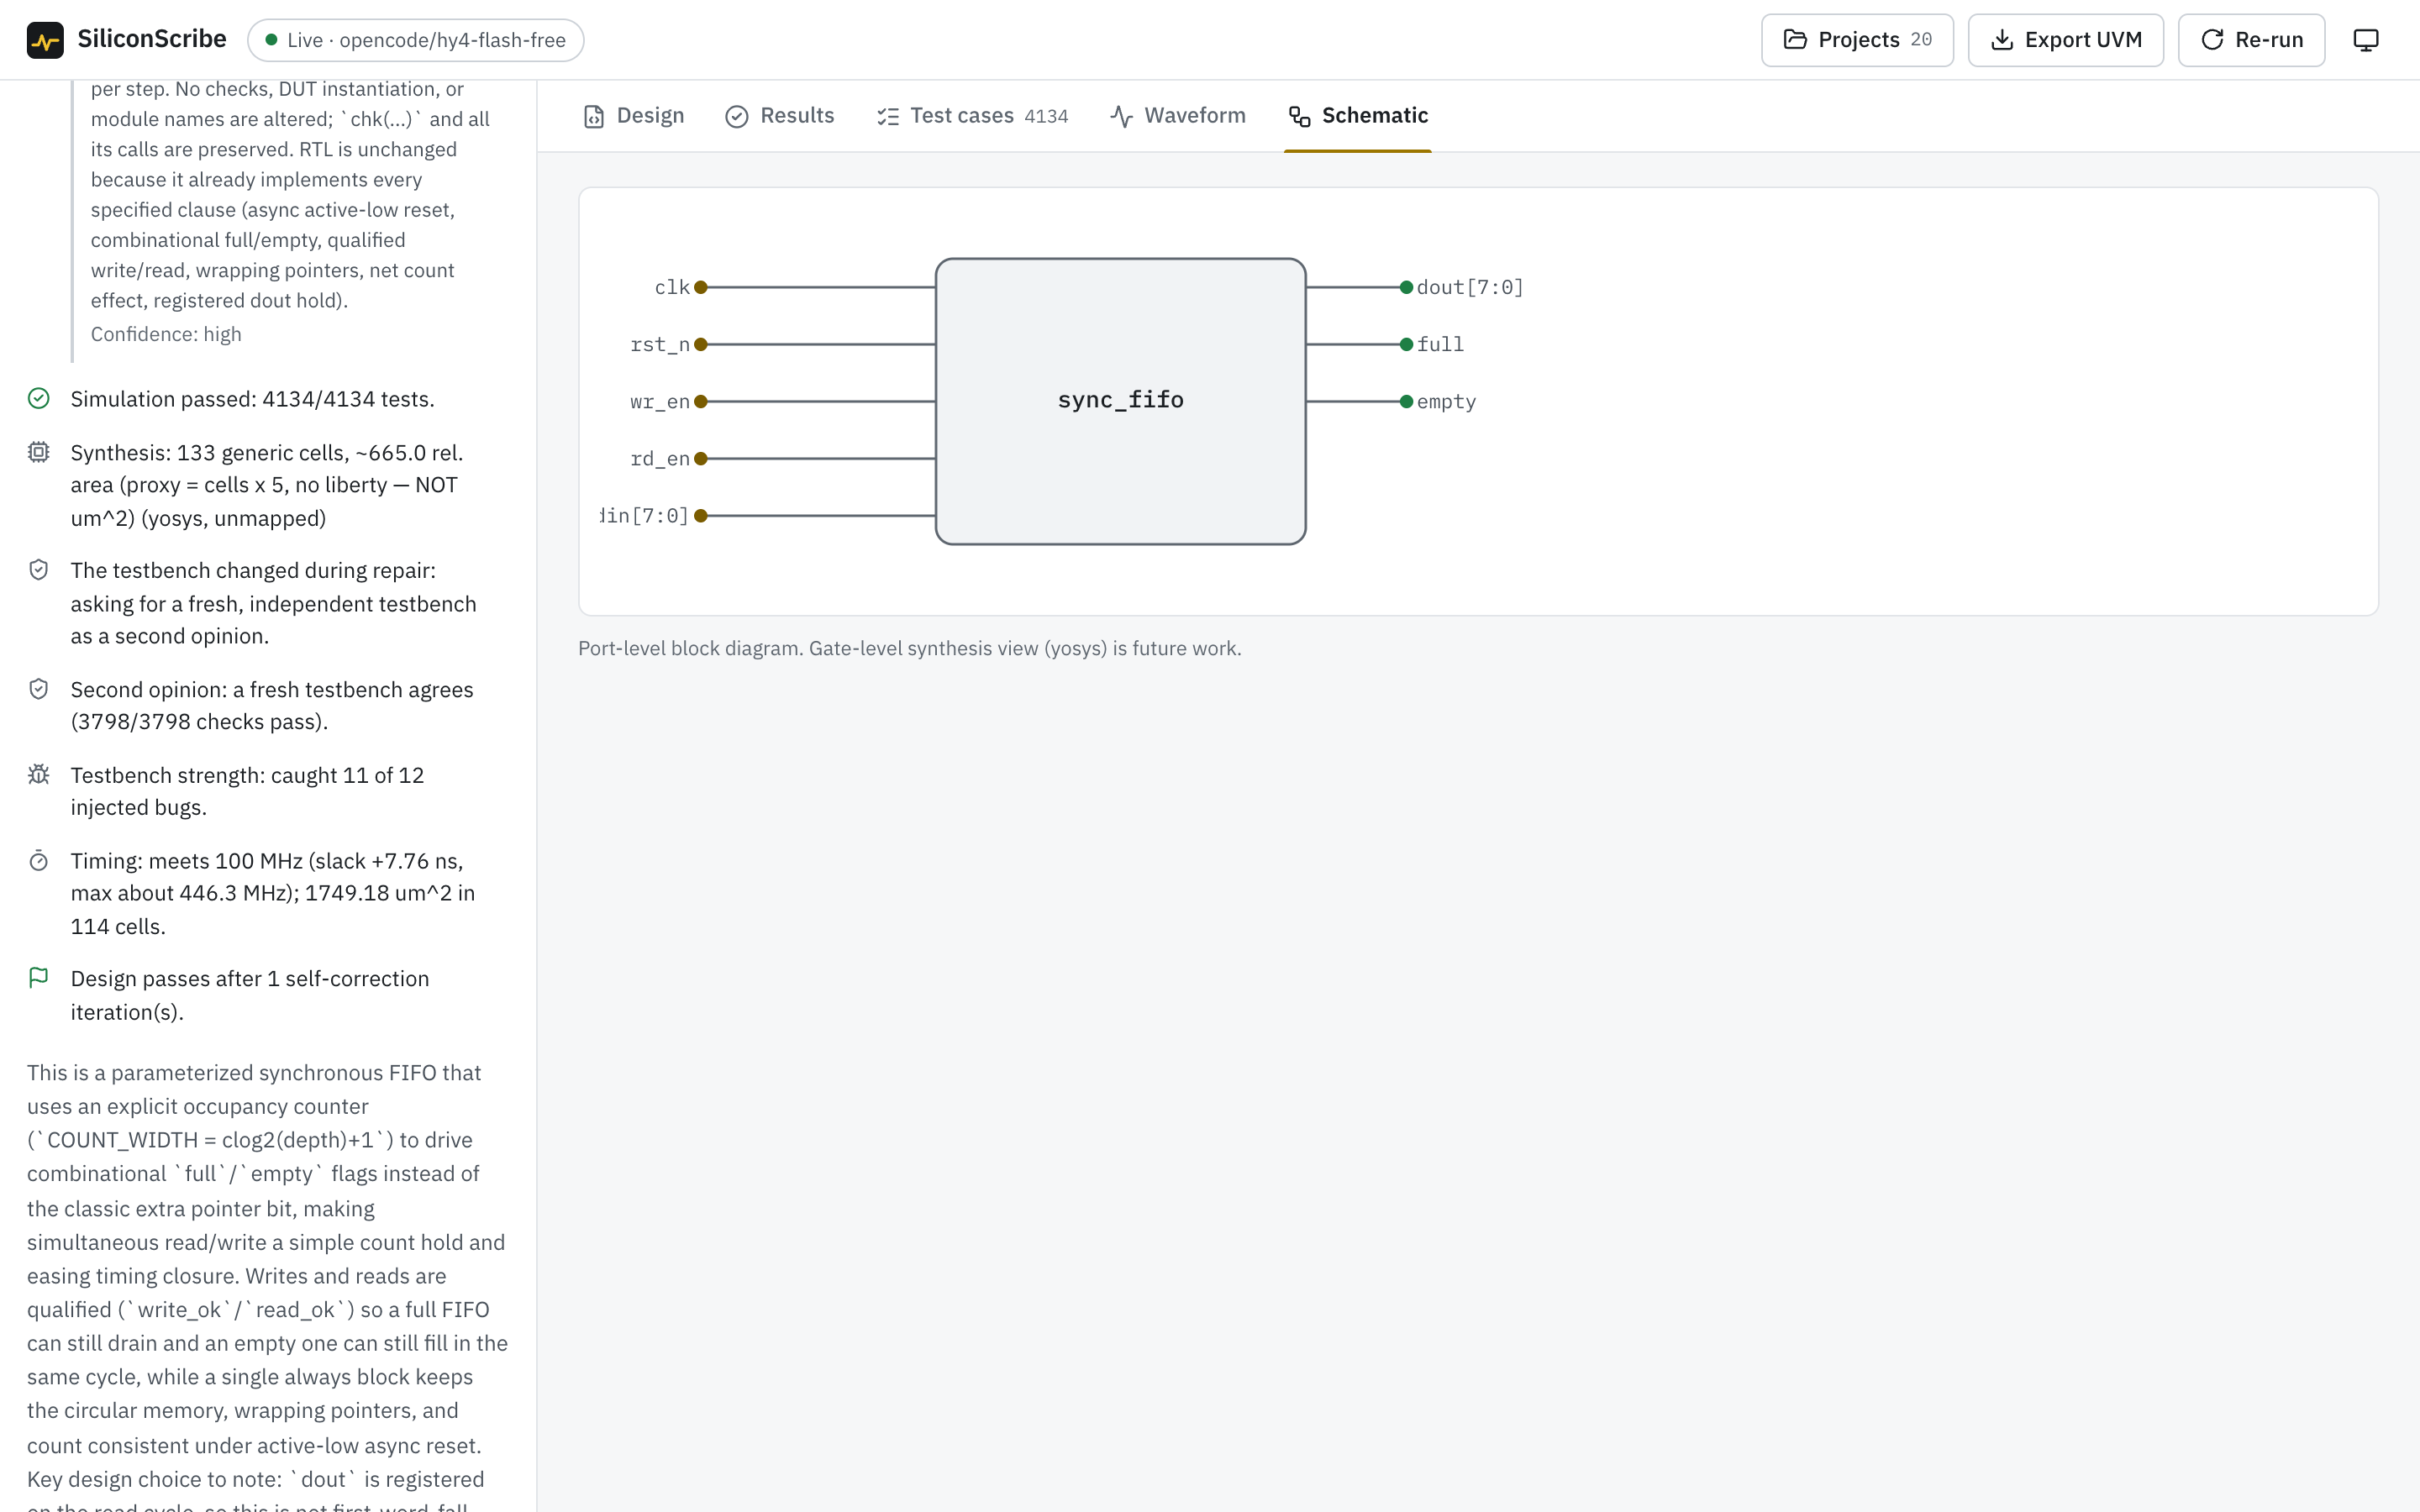
\includegraphics[width=0.92\textwidth]{s11_schematic.png}
\caption{The Schematic tab: a port-level block diagram of the FIFO.}
\end{figure}

\begin{figure}[H]
\centering
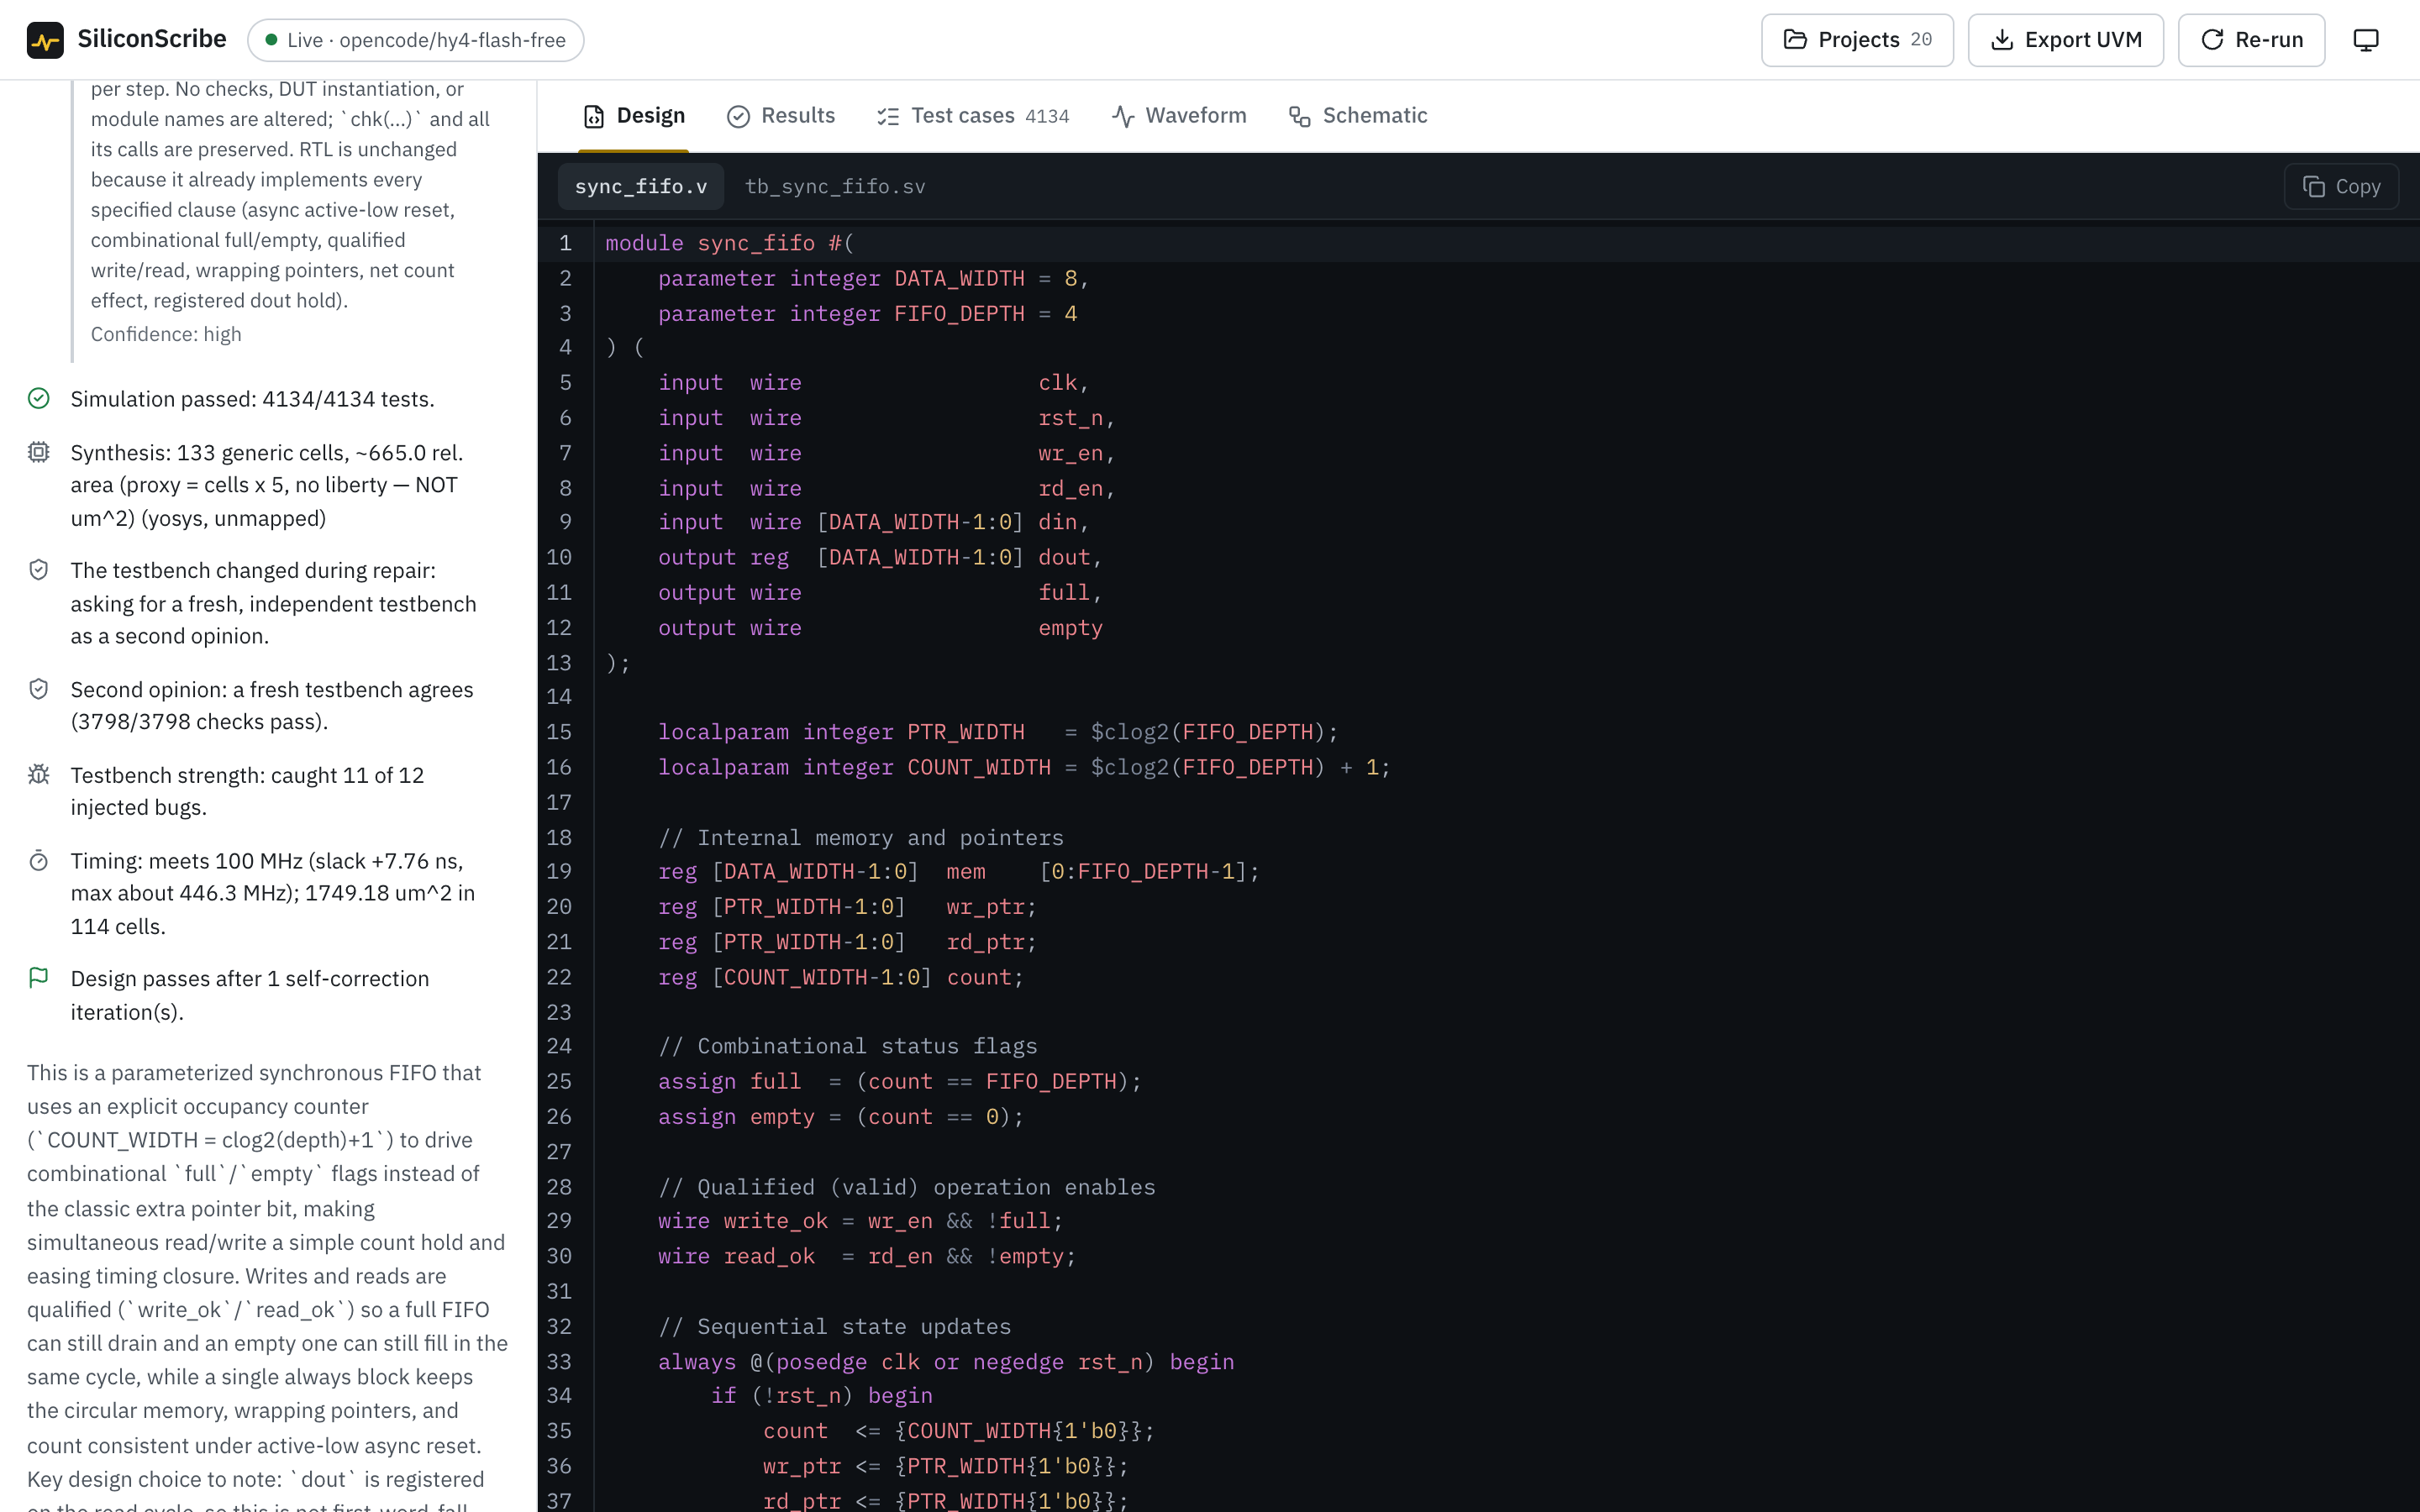
\includegraphics[width=0.92\textwidth]{s12_design_tab.png}
\caption{The Design tab: generated RTL and testbench in editable code editors.}
\end{figure}

\section{Editing and re-running}

You can edit the RTL or testbench directly in the Design tab, then press \textbf{Re-run} to simulate once more without the AI. This is useful for trying your own fix, or for checking that a deliberate bug is caught: change \code{count + 1'b1} to \code{count + 2'd2} in a counter, press Re-run, and the Test cases and Waveform tabs show the failures at once. Re-run clears strength, timing, the second opinion and ``Written by'', because those described the previous code.

\begin{figure}[H]
\centering
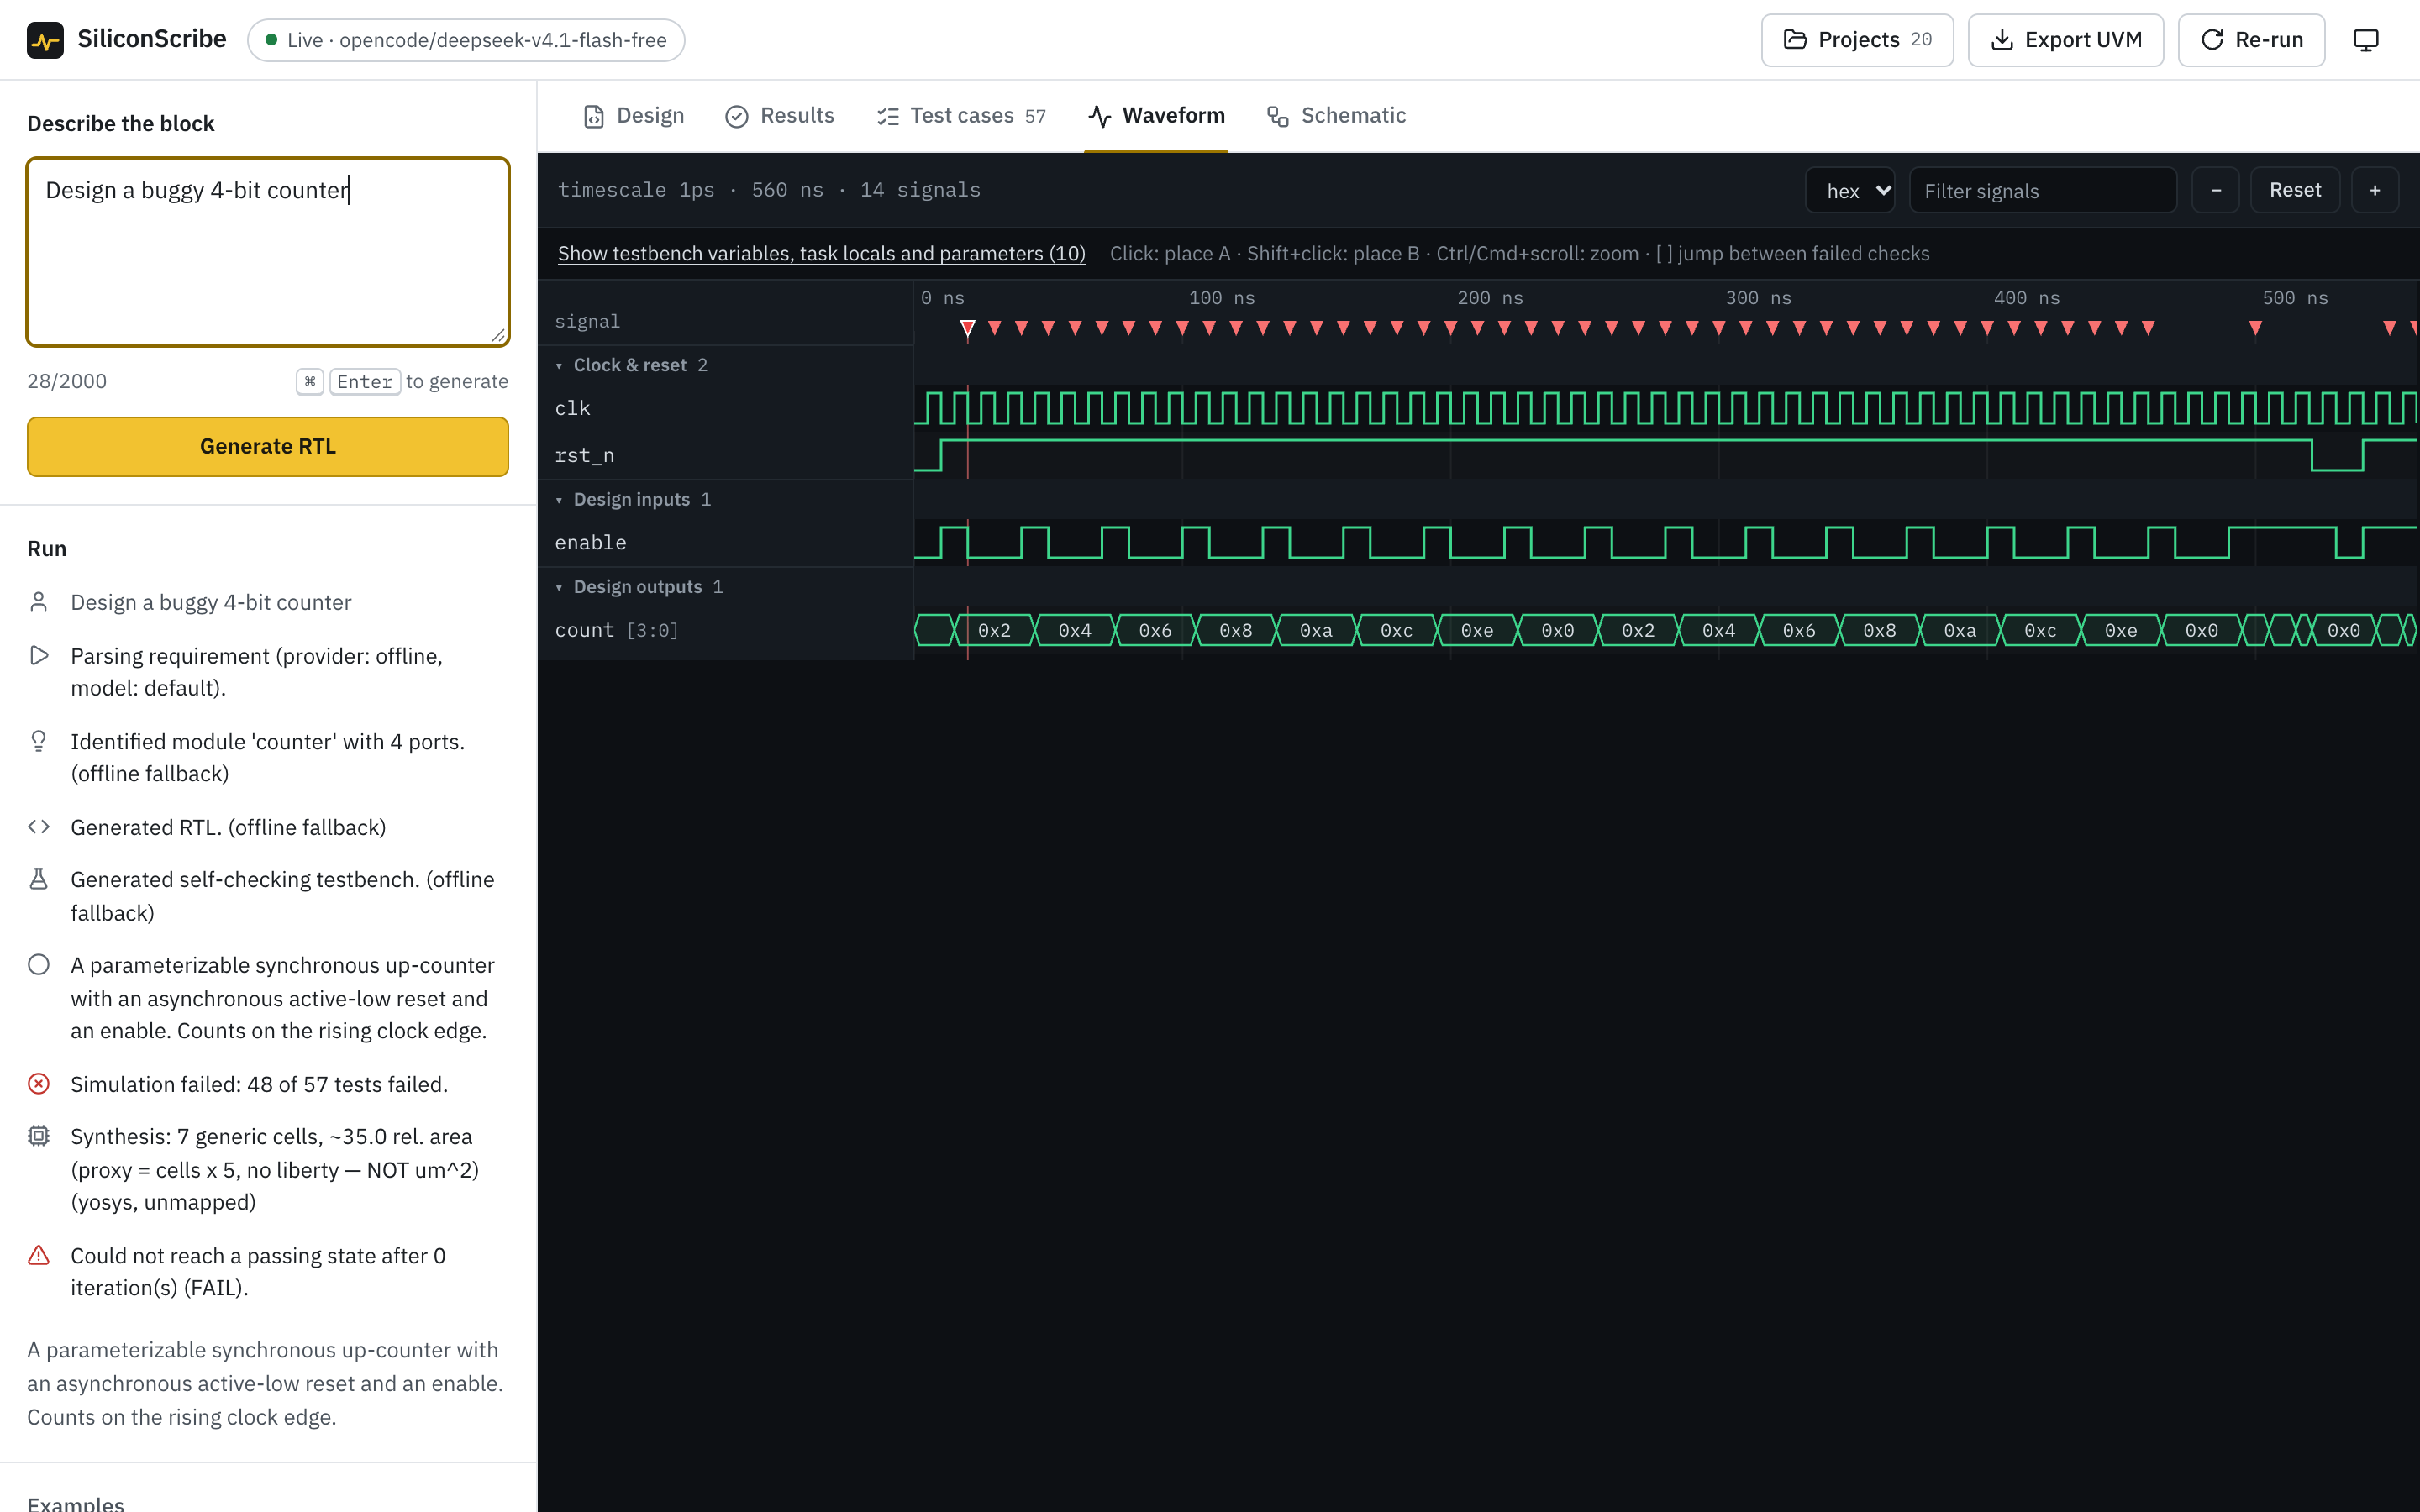
\includegraphics[width=0.92\textwidth]{s13_failure_waveform.png}
\caption{Waveform of the scripted buggy-counter demo (offline): each red marker is a failed check (48 of 57).}
\end{figure}

\section{Projects, theme, UVM export and Stop}

\textbf{Projects} opens a menu of saved runs (newest first), each with its module name, status and prompt, and \textbf{Open} and \textbf{Delete} buttons (Delete asks first). Before the first run, the start screen also lists recent projects. The theme button cycles between system (follows the computer's setting), light and dark; an explicit choice is remembered in the browser. \textbf{Export UVM} downloads the 16-file UVM bundle as a zip (export only: it is not simulated). \textbf{Stop} cancels a running generation.

\begin{figure}[H]
\centering
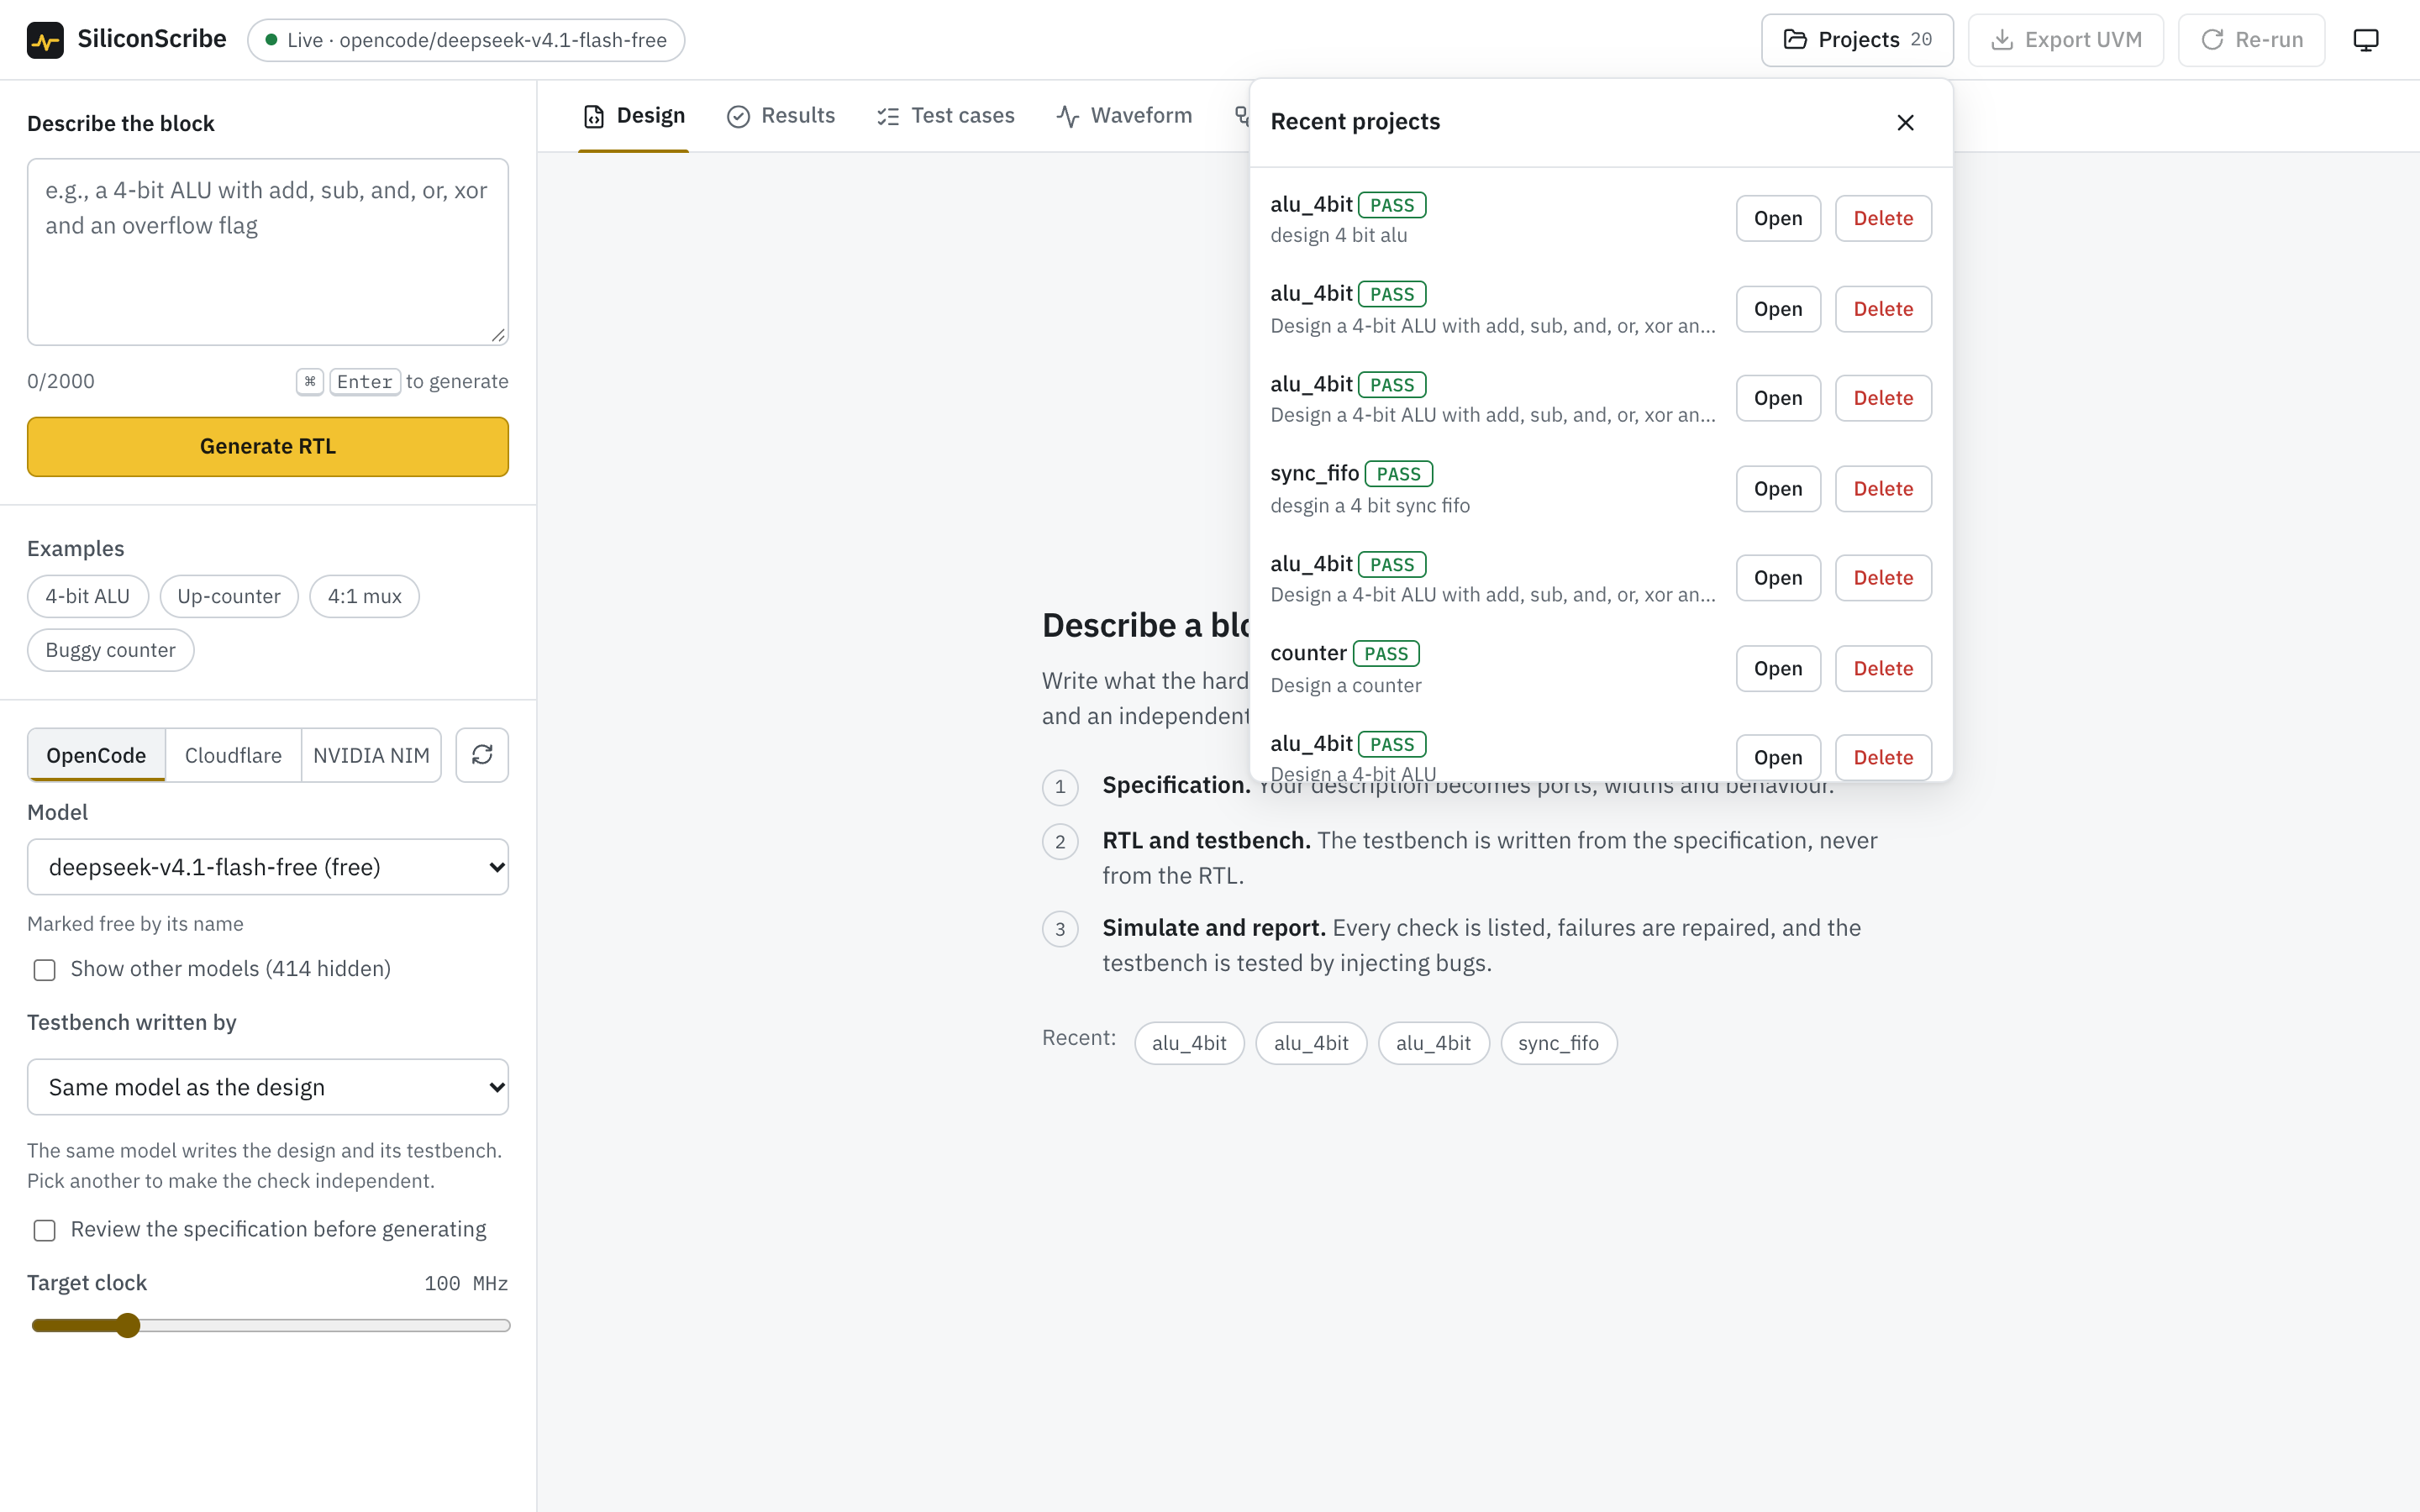
\includegraphics[width=0.92\textwidth]{s14_projects_menu.png}
\caption{The Projects menu listing saved runs.}
\end{figure}

\begin{figure}[H]
\centering
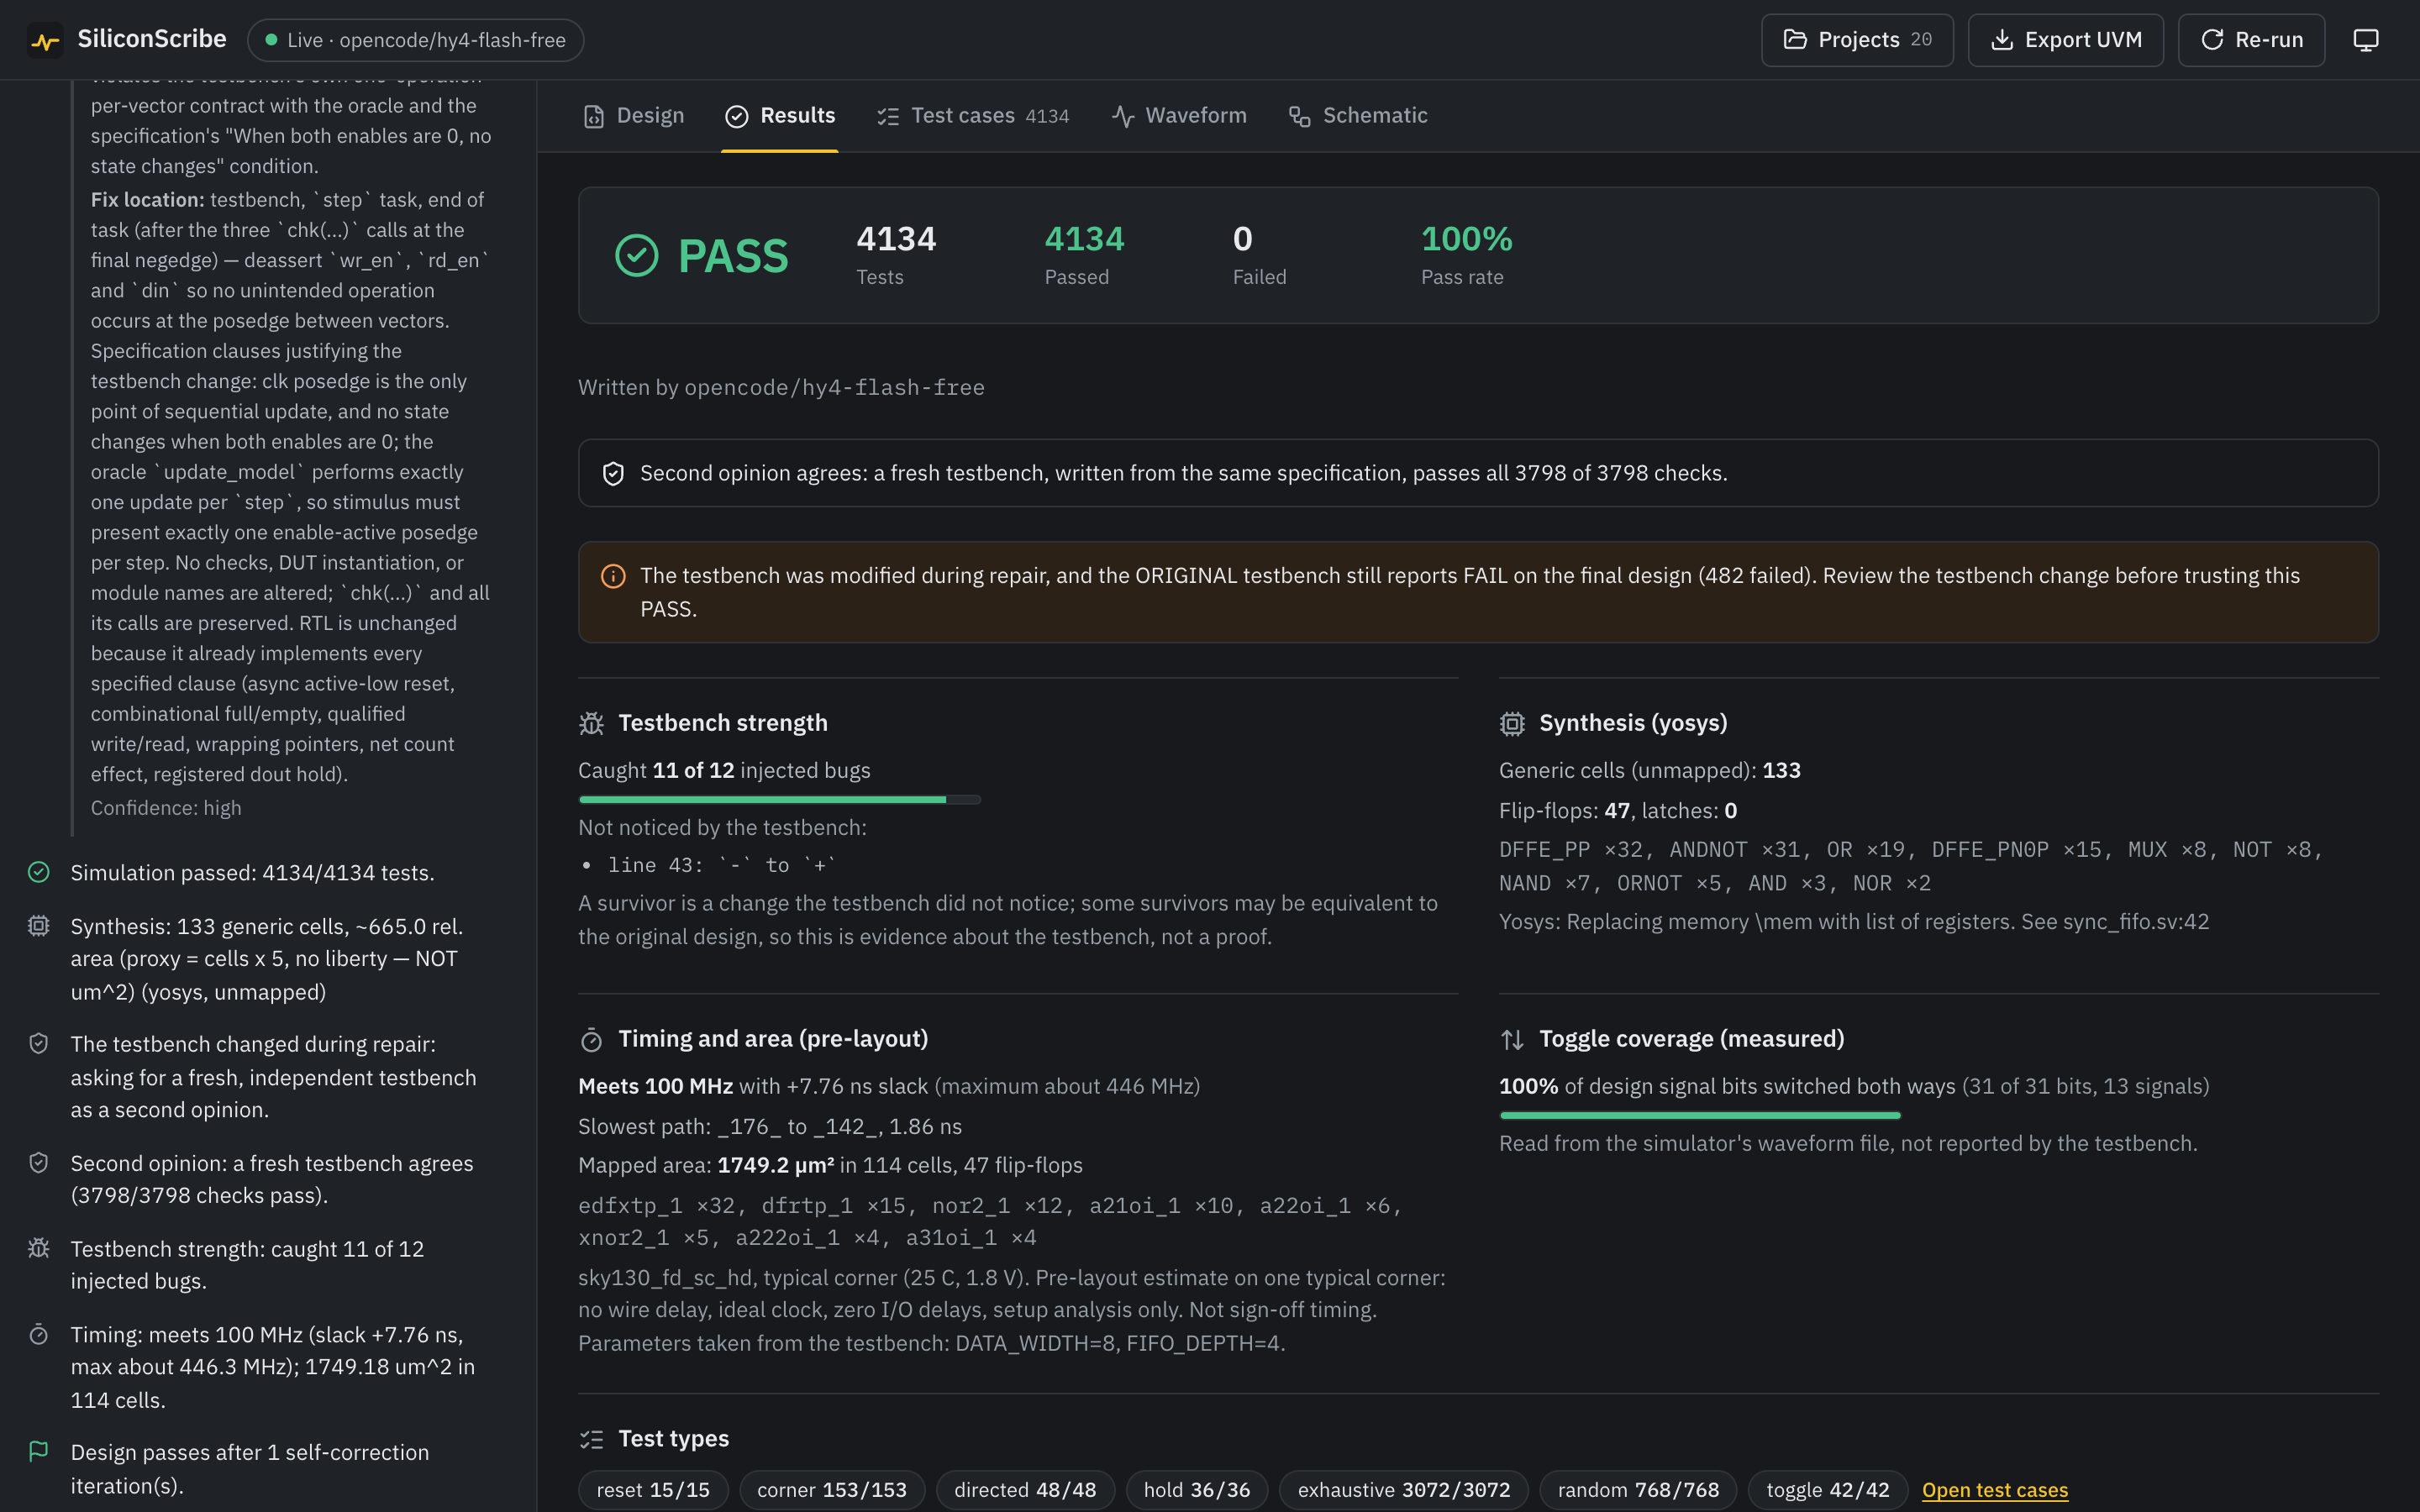
\includegraphics[width=0.92\textwidth]{s16_dark_theme.png}
\caption{The Results tab in the dark theme.}
\end{figure}

\begin{figure}[H]
\centering
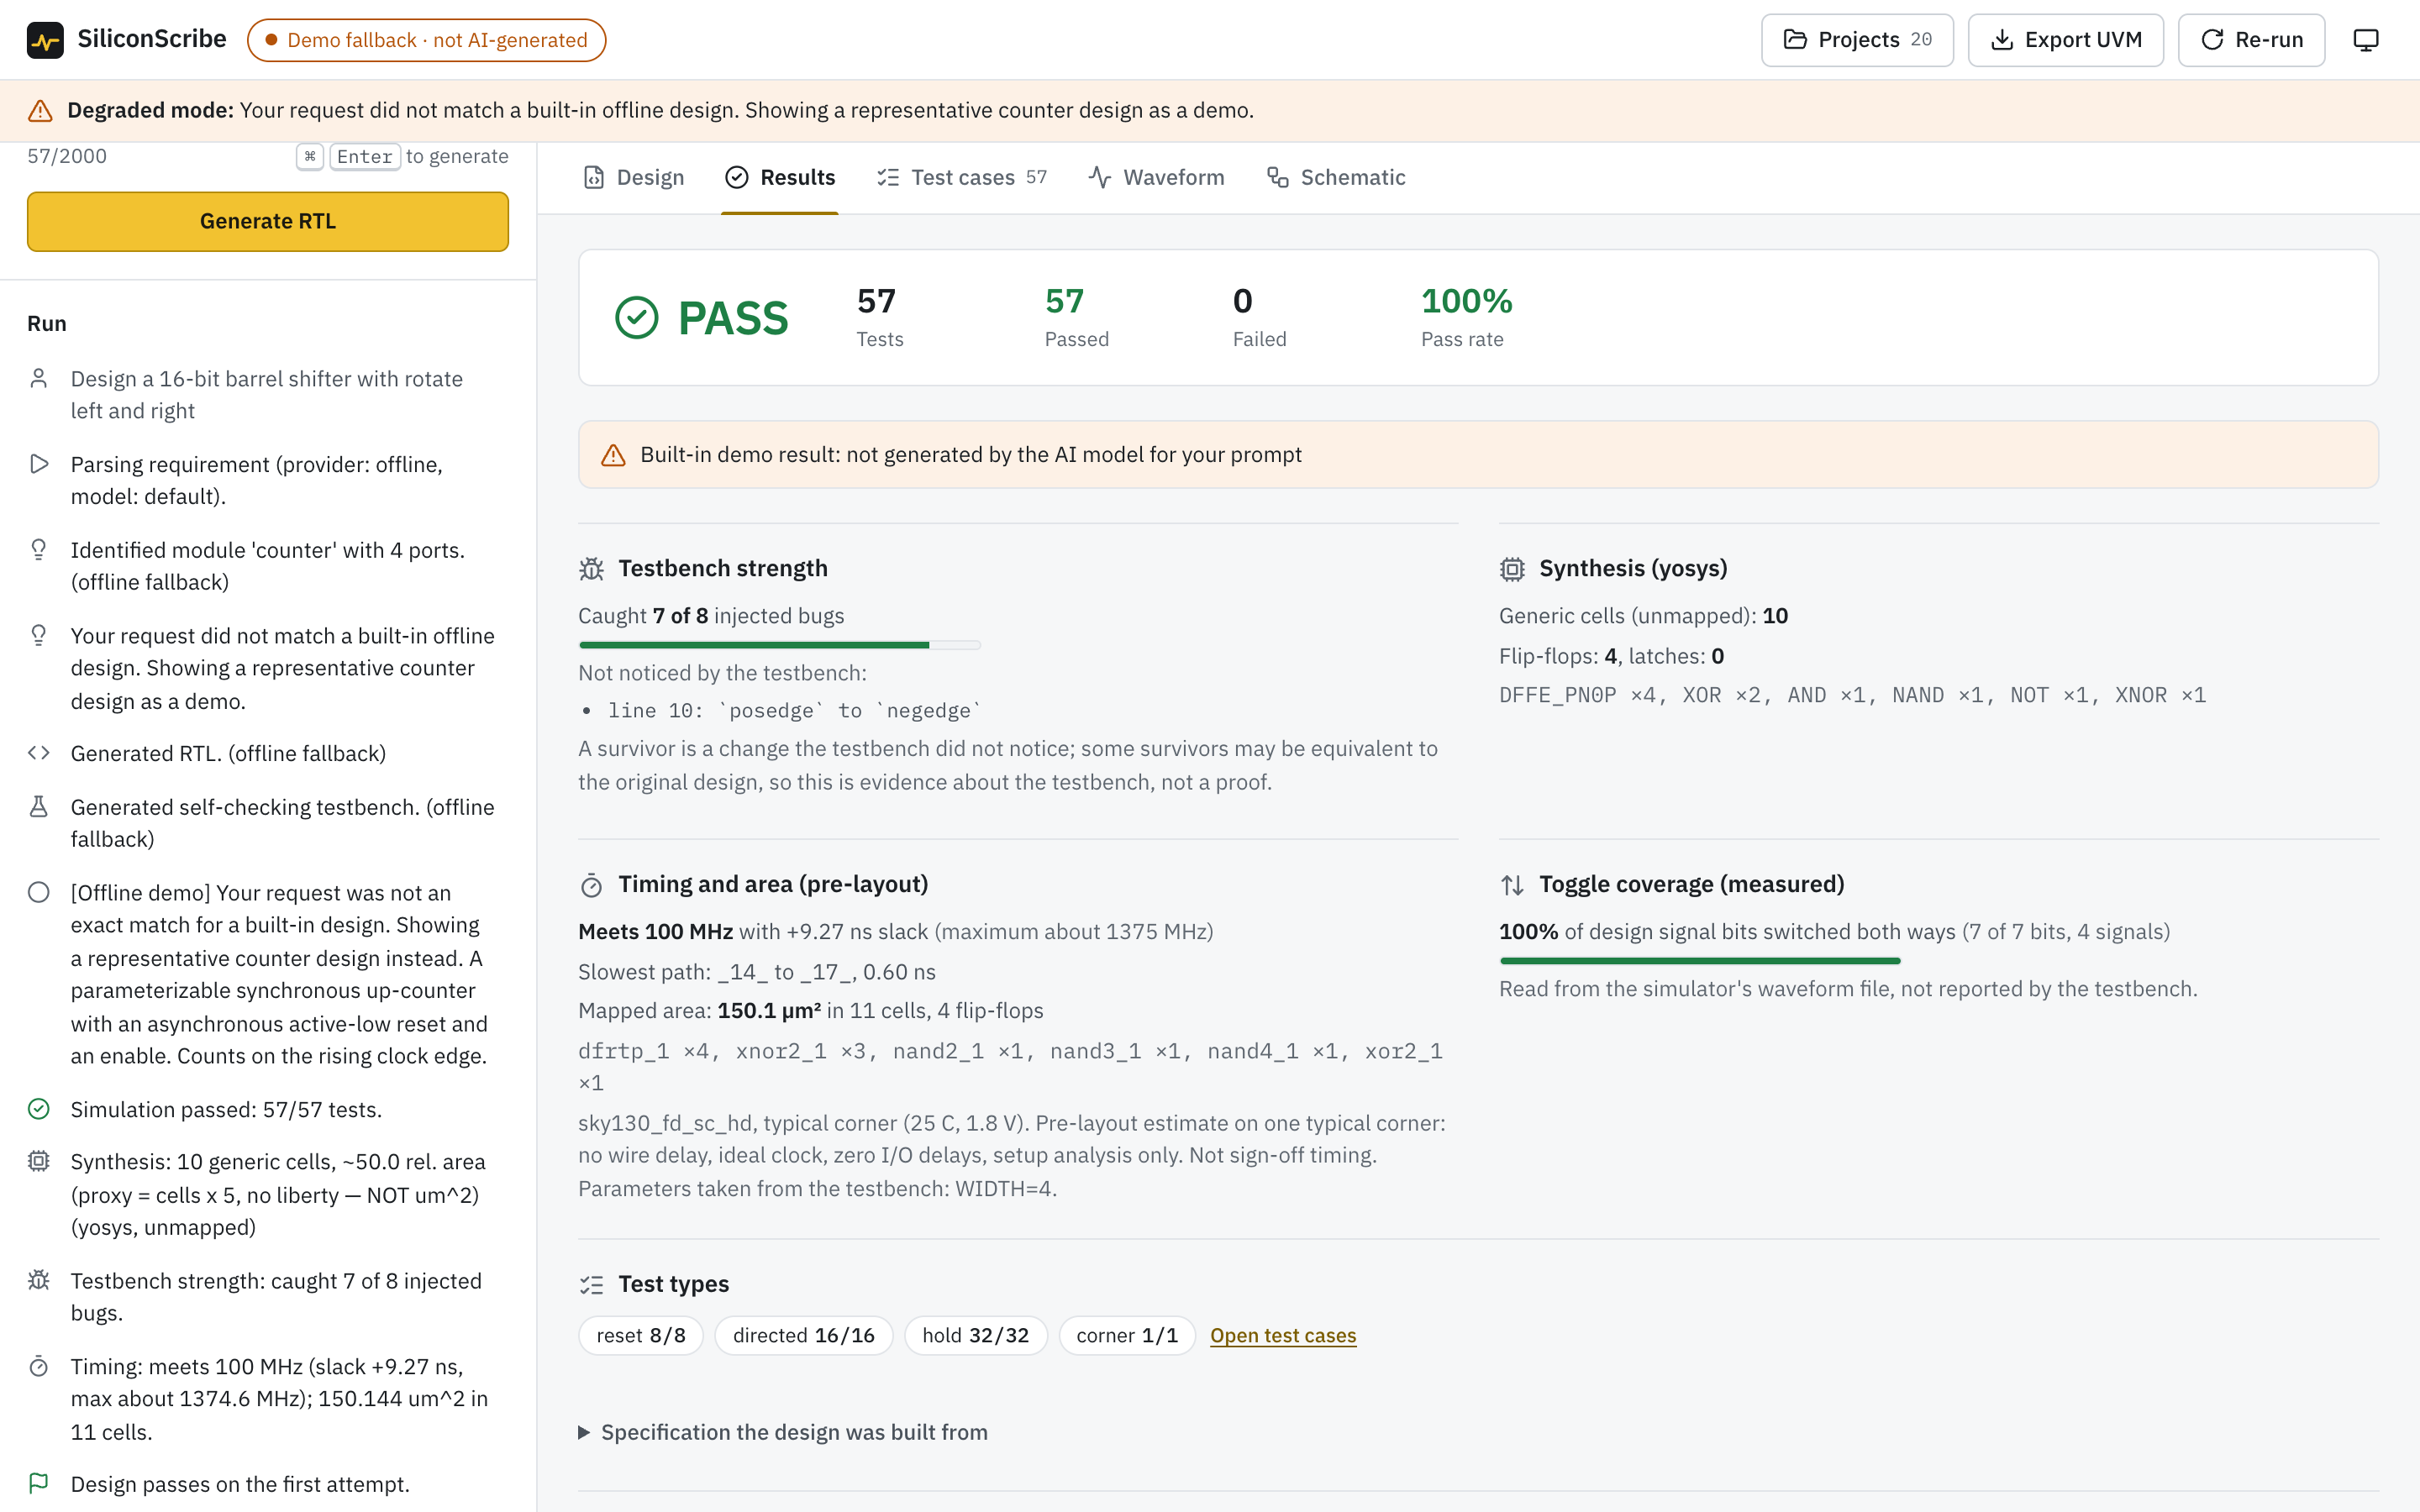
\includegraphics[width=0.92\textwidth]{s15_offline_demo.png}
\caption{A run that fell back to the built-in demo is labelled as such: the ``Degraded mode'' banner and ``Built-in demo result: not generated by the AI model for your prompt''.}
\end{figure}

% ---------------------------------------------------------------------------
\chapter{Testing and Quality}
\label{ch:testing}

\section{Verification commands}

These are the checks behind the numbers in this guide (final run: 19 Nov 2026). Run them from the project folder; none of them needs a key except the last.

\begin{lstlisting}[style=plain]
cd backend
PATH="$HOME/.local/bin:$PATH" OFFLINE_MODE=1 python3 -m pytest tests/ -q   # 436 passed
python3 tools/mutation_sweep.py                       # 27 of 27 injected bugs caught
PATH="$HOME/.local/bin:$PATH" python3 tools/verify_mapping.py   # 19 of 19 equivalent
python3 evaluation/independent/run.py                 # every evaluated design vs. its reference
PATH="$HOME/.local/bin:$PATH" python3 evaluation/independent/strength.py   # the references' own strength

cd ../frontend
npm test                                              # 211 passed (Vitest)
npm run build                                         # TypeScript check + production build
\end{lstlisting}

\begin{description}
  \item[pytest] 436 backend tests in 31 test files. They use a temporary workspace (the \code{_isolated_workspace} fixture in \file{tests/conftest.py}), so they never touch your real \file{projects.db}. Tests that need Icarus, Yosys or OpenSTA are skipped automatically if the tool is missing; Cloudflare and NIM are tested against small fake servers, not the internet.
  \item[Mutation sweep] Injects 27 known bugs into the built-in designs and checks that the built-in testbenches catch every one.
  \item[Mapping verification] The checks of Chapter~\ref{ch:timing}: gate-level simulation agrees with the RTL, area and cells recount, minimum period independent of the target. Each design says OK or REFUSED (with a reason).
  \item[Independent references] Hand-written reference testbenches, not written by any model, for the 14 evaluated designs. All 14 final designs were correct (no false PASS). \file{strength.py} runs \emph{every} mutant (not a sample of 12) against each reference; the references caught every mutant except equivalent ones, unreachable code, or behaviour the prompt does not define.
  \item[Frontend] 211 Vitest tests; \code{npm run build} runs the TypeScript compiler (clean) and the production build.
  \item[Accessibility] An automated axe-core audit of every tab, both themes, for a passing and a failing run: 0 violations. Its structural rules also run in the test suite. This is an automated audit, not a user study.
  \item[Tests of the tests] The newest components were broken on purpose, one behaviour at a time, and the tests had to fail.
\end{description}

\section{The preflight check}

Before a demo, \file{tools/preflight.py} checks everything the demo needs: the tools and their versions, the cell library, the model, the offline demo and the saved results. Each line is OK, WARN or FAIL, and the last lines say which rung of the fallback ladder (live model, offline demo, saved results) is usable. Without \code{--live} it makes no model call; with \code{--live} it makes one tiny call. It never writes to the projects database.

\begin{lstlisting}[style=plain]
cd backend
PATH="$HOME/.local/bin:$PATH" env -u OFFLINE_MODE LLM_PROVIDER=opencode-app \
  LLM_MODEL=deepseek-v4.1-flash-free LLM_TIMEOUT_SECONDS=360 python3 tools/preflight.py --live
\end{lstlisting}

The final run reported 0 failures and 0 warnings, with all three fallback rungs ready.

\section{What the test files protect}

\begin{center}
\small
\begin{tabularx}{\textwidth}{@{}>{\raggedright\arraybackslash}p{5.2cm}X@{}}
\toprule
\textbf{File(s)} & \textbf{Guards against} \\
\midrule
\file{test_orchestrator.py}, \file{test_edge_cases.py} & Broken repair loop, fallback rules, guards (anti-cheat, no-op, oscillation), compiler repairs, odd inputs. \\
\file{test_verdict_integrity.py}, \file{test_simulator.py} & A wrong verdict: misplaced or non-numeric summaries, zero checks, FAIL lines under ``Failed: 0'', killed runs, forged summaries in the RTL, system tasks not on the allow-list, narrow testbench wires, hangs. \\
\file{test_sandbox.py} & File access from Verilog, string tricks, the real exploit, environment scrubbing, output cap. \\
\file{test_verification_quality.py}, \file{test_mutation.py} & Testbenches that cannot fail; the strength stage (operators, protected regions, scoring, time budget). \\
\file{test_trust_signals.py}, \file{test_toggle_coverage.py} & The weak-evidence and weak-testbench warnings; measured toggle coverage. \\
\file{test_independent_testbench.py}, \file{test_spec_review.py} & The separate testbench model rules, the second opinion, the reviewed specification and its bounds. \\
\file{test_timing.py}, \file{test_verify_mapping.py}, \file{test_synthesis_metrics.py}, \file{test_yosys_warnings.py} & The timing stage (parsing, parameter overrides, clocks from the netlist, every refusal) and its checker; generic synthesis metrics; Yosys warnings shown with file names only. \\
\file{test_model_catalog.py}, \file{test_model_switching.py}, \file{test_model_routing.py}, \file{test_opencode_provider.py} & The Model menu, per-run model choice and routing, model-id validation, keys never leaking, the OpenCode app provider. \\
\file{test_llm_parsing.py}, \file{test_error_messages.py} & Fragile parsing of model answers; plain, safe error messages. \\
\file{test_api.py}, \file{test_stream_persistence.py}, \file{test_disconnect.py} & Routes, streaming, rate limit, saving streamed runs, a closed browser tab stopping further stages. \\
\file{test_check_parser.py}, \file{test_vcd_parser.py}, \file{test_vcd_roles.py}, \file{test_linter.py}, \file{test_models.py} & Check rows, waveform parsing and signal roles, lint, data shapes. \\
\file{test_preflight.py}, \file{test_evaluate_live.py} & The demo preflight and the live-evaluation recorder. \\
\bottomrule
\end{tabularx}
\end{center}

\begin{keyidea}
The most important tests are the ones that prove a check can fail: mutation tests of the testbenches, sabotaged netlists for the timing checker, broken components for the test suite itself. A test suite that only checks that correct designs pass proves very little.
\end{keyidea}

% ---------------------------------------------------------------------------
\chapter{Configuration Reference}
\label{ch:config}

All of these are read by the backend, from \file{backend/.env} or the environment.

\begin{center}
\small
\begin{longtable}{@{}>{\ttfamily\raggedright\arraybackslash}p{5.0cm}p{10.0cm}@{}}
\toprule
\textrm{\textbf{Variable}} & \textbf{Effect} \\ \midrule \endhead
OFFLINE\_MODE & 1/true/yes/on forces the offline provider. \\
LLM\_PROVIDER & \code{opencode-app}: use the installed OpenCode app. \\
LLM\_MODEL & Default model (where the Model menu starts), for example \code{deepseek-v4.1-flash-free}. \\
OPENCODE\_AGENT & OpenCode agent used for each call (default \code{plan}, read-only). \\
CLOUDFLARE\_ACCOUNT\_ID, CLOUDFLARE\_API\_TOKEN & Turn on the Cloudflare tab. \\
NVIDIA\_NIM\_API\_KEY, NVIDIA\_NIM\_BASE\_URL & Turn on the NVIDIA NIM tab (key starts \code{nvapi-}). \\
OPENCODE\_API\_KEY / ZEN\_API\_KEY, ZEN\_MODEL, OPENCODE\_BASE\_URL & OpenCode Zen as the default provider instead of the app. \\
NVIDIA\_API\_KEY, NVIDIA\_BASE\_URL & Older single-model NVIDIA default provider (not used by the NIM tab). \\
OPENAI\_API\_KEY, OPENAI\_BASE\_URL, LLM\_MINI\_MODEL & OpenAI, or any compatible gateway when a base URL is given. \\
LLM\_MODEL\_INTENT, \_RTL, \_TESTBENCH, \_EXPLAIN, \_FIX & Per-stage model routing for the default provider (a model chosen in the menu still wins). \\
LLM\_TIMEOUT\_SECONDS & Per-call timeout (default 120; 360 for the free models in the demo). \\
LLM\_MAX\_TOKENS & Answer budget (default 8192). \\
STRENGTH\_ENABLED, STRENGTH\_MAX\_MUTANTS, STRENGTH\_BUDGET\_SECONDS & Testbench strength on/off (default on), mutants per run (12), time budget (40 s). \\
TIMING\_ENABLED & Timing and area estimate on/off (default on; needs the tools and library). \\
SECOND\_OPINION\_ENABLED & Second opinion on/off (default on). \\
SIM\_MAX\_CONCURRENT, SIM\_MAX\_MEMORY\_MB & Simulations at once (2); memory cap per simulation (1024 MB, Linux only). \\
CORS\_ALLOW\_ORIGINS & Extra exact browser origins allowed to call the API (comma-separated, no wildcards). \\
TRUST\_PROXY\_HEADERS & 1 only behind a trusted reverse proxy, so the rate limit uses the forwarded address. \\
ADMIN\_TOKEN & Enables \code{/api/admin/cleanup}; sent as the \code{X-Admin-Token} header. \\
VITE\_API\_BASE & Frontend: backend address if not served from the same origin. \\
\bottomrule
\end{longtable}
\end{center}

% ---------------------------------------------------------------------------
\chapter{Troubleshooting}
\label{ch:trouble}

\begin{center}
\small
\begin{longtable}{@{}p{4.6cm}p{10.4cm}@{}}
\toprule
\textbf{Symptom} & \textbf{Cause and fix} \\ \midrule \endhead
Status ERROR, ``Compilation failed'' & The code does not compile. Read the error line in the log; the loop repairs wire/reg and disable/return automatically and asks the model for anything else. \\
``Rejected by sandbox policy'' & The code uses a file or system task (\code{$fopen}, \code{$readmemh}, \code{`include}, \ldots) or a task not on the allow-list. Remove it. \\
Status ERROR, ``No valid summary'' & The testbench did not print whole-line \code{Passed:} and \code{Failed:} numbers, often because its own watchdog fired first. Re-run with a fresh testbench or another model. \\
``The model you chose (\ldots) could not be used'' & That model hit its limit, timed out, was refused or is unknown. Pick another model from the Model menu. Your run is not replaced by the demo. \\
``The AI model did not answer in time'' & Free models can take minutes per step. Try again, pick another model, or raise \code{LLM_TIMEOUT_SECONDS}. \\
``free usage limit has been reached'' & The free quota is used up; it resets daily. Switch model or provider, or use the offline demo or a saved project. \\
Cloudflare or NVIDIA NIM tab says ``not set up'' & The key is missing or malformed in \file{backend/.env}. Fix it and restart the backend. \\
Cloudflare HTTP 403, code 5035 & That model is not allowed on the Workers Free plan. Pick another. \\
GitHub Copilot is not in the menu & Connect it in the OpenCode app with \code{/connect}, press the refresh button, tick ``Show other models''. \\
``LLM became unavailable mid-run'' & The provider failed after the run had started producing your design. Retry; the app refuses to swap in a demo design at this point. \\
Banner ``Degraded mode'' & The default provider failed before anything was generated, so the run used built-in designs and says so. Check the model and network. \\
No ``Timing and area'' section & Yosys, OpenSTA or \file{backend/pdk/sky130hd_tt.lib} is missing, or the run did not PASS. Start the backend with \code{PATH="$HOME/.local/bin:$PATH"}. \\
Timing shows a reason instead of a number & The design has tri-states, latches, a combinational loop, a derived or gated clock, or no logic cells. This is a deliberate refusal (Chapter~\ref{ch:timing}). \\
HTTP 429 & More than 20 requests in a minute from your address. Wait a minute. \\
Status TIMEOUT & The testbench never calls \code{$finish}, or runs too long. Check loops; the limit is 1--120 s (30 s from the UI). \\
The browser cannot reach the API from another address & CORS allows local addresses only. Add the exact origin with \code{CORS_ALLOW_ORIGINS}. \\
\code{simulator: false} in /health & Icarus is not on the PATH. Install it and restart. \\
\bottomrule
\end{longtable}
\end{center}

% ---------------------------------------------------------------------------
\chapter{Extending the Project}
\label{ch:extend}

\section{Adding an LLM provider}
Any OpenAI-compatible service works as the default provider with no code change: set \code{OPENAI_API_KEY}, \code{OPENAI_BASE_URL} and \code{LLM_MODEL}. To add it as a tab of the Model menu (like Cloudflare and NIM), give its ids a unique prefix, add a \code{..._config}, a catalogue reader and a \code{..._status} function in \file{model_catalog.py} that read the key only from the environment and never return it, add a small subclass of \code{OpenAIProvider} in \file{llm_service.py}, route the prefix in \code{get_provider}, add it to \code{list_models}, and add a fake server for its tests. Keep every id inside \code{MODEL_ID_RE}.

\section{Adding a built-in design}
In \file{offline_designs.py}, add a spec, an RTL string starting with \code{_marker("key")}, a self-checking testbench ending with the summary lines, and an explanation; register it in \code{DESIGNS} and add keywords to \code{_KEYWORDS}. Then add mutants for it in \file{tests/test_verification_quality.py} and \file{tools/mutation_sweep.py} to prove its testbench can fail, and run \file{tools/verify_mapping.py} on it.

\section{Adding a compiler repair}
Write a function like \code{_repair_disable_functions} that only acts when the compiler log contains a specific, unambiguous message, call it from \code{_compiler_repairs}, return a structured diagnosis, and add a test with the real compiler message.

\section{Adding a pipeline stage or UI panel}
Yield a new event from \code{pipeline_events} with its own \code{stage} name, add the stage to \code{StreamEvent} in \file{frontend/src/types.ts}, handle it in \code{startRun}, and render it in a component. Keep extra stages non-fatal, as the explanation, strength, timing and second-opinion stages are.

% ---------------------------------------------------------------------------
\chapter{Why It Is Built This Way}
\label{ch:why}

\begin{description}[style=nextline]
  \item[Why generate the testbench from the specification and not the RTL?]
  So a wrong design and its testbench cannot simply agree. It removes the most direct form of circular checking.
  \item[Why offer a separate testbench model, but not by default?]
  Two models reading the specification independently can catch a misreading one model would make twice. But it costs an extra call, and with the free models tried it was not reliable enough to be the default. As an option it makes disagreements visible instead of quietly repaired.
  \item[Why a second opinion after a repair?]
  A PASS that appears only after the testbench was rewritten might come from a relaxed check. A fresh testbench from the same specification is cheap independent evidence; disagreement is the signal.
  \item[Why measure testbench strength on every PASS?]
  A PASS from a testbench that cannot catch bugs means little. Injecting small bugs and counting how many are caught is the classic, direct way to ask.
  \item[Why only toggle coverage?]
  It can be measured honestly from the VCD the simulator already writes. Line and branch coverage need a simulator that instruments the code; Verilator was tried and could not build most of the generated testbenches.
  \item[Why Icarus Verilog and not a commercial simulator?]
  It is free, open source, scriptable and installable anywhere, which fits a zero-budget project. The trade-off is limited SystemVerilog support (hence the Icarus-safe prompts and repairs, and why UVM is export-only).
  \item[Why a pre-layout timing estimate and not final timing?]
  Sign-off needs place and route, extracted wire delays, a real clock tree and several corners. That is a full physical-design flow. A pre-layout estimate on real sky130 cells already answers the useful early question, and every limit is printed next to the number.
  \item[Why refuse some designs instead of timing them?]
  For tri-states, latches, loops and derived clocks this simple set-up would time a different circuit or an undefined one. A reason is honest; a number would not be.
  \item[Why fix compiler errors without the AI?]
  When the compiler names the exact problem, the fix is mechanical. A deterministic repair is instant, free and always correct for that case; the AI is kept for real reasoning.
  \item[Why read model catalogues live?]
  Model names change and models are retired (one NIM model returned HTTP 410 three days before the final check). A hand-written list goes stale.
  \item[Why keep keys only in \texttt{backend/.env}?]
  A key typed into a web page can leak through the browser, logs or screenshots. The backend is the only part that needs it.
  \item[Why Server-Sent Events and not WebSockets?]
  The data only flows one way (server to browser) during a run. SSE is plain HTTP, works through proxies and hosting platforms, and needs no extra protocol.
  \item[Why SQLite?]
  Zero setup and zero cost for a single server. The report's scaling path moves to PostgreSQL for many users.
  \item[Why disable hidden reasoning by default?]
  Reasoning tokens use the same budget as the answer. In a live test a model spent all 8192 tokens thinking and returned nothing.
  \item[Why fall back to offline only before the first live success, and never for a model you chose?]
  Before anything is generated, a labelled demo is better than an error. After your design exists, or when you deliberately picked a model, swapping in a demo would be dishonest, so the run fails with a plain reason instead.
  \item[Why plain \texttt{def} handlers instead of \texttt{async def}?]
  Simulations block while waiting for a subprocess. In \code{async def} they froze the whole server; in \code{def} FastAPI runs them in a thread pool.
\end{description}

\section{Limitations to state openly}

\begin{enumerate}
  \item One model writes the design and the testbench unless a separate testbench model is chosen (common-mode risk).
  \item The specification is written by the model unless you review it.
  \item Testbench strength is a sample of up to 12 one-token (syntactic) mutants; survivors may be equivalent.
  \item Only toggle coverage is measured; there is no line or branch coverage, no assertions and no formal checks.
  \item Timing is pre-layout on one typical corner: no wires, ideal clock, setup only, no power. It is not sign-off.
  \item Free models are slow (minutes per run) and quota-limited.
  \item The sandbox is defence in depth, not a jail or a container boundary.
  \item The evaluation used small blocks (under about 100 lines), one run per prompt, mainly one model.
  \item GitHub Copilot ``auto'' cannot name the model that wrote a result.
  \item The UVM bundle is exported, not compiled or run.
  \item One server, in-process rate limiter, SQLite, and a local single-user model provider: not a multi-user production service.
\end{enumerate}

\section{Future work}

\begin{enumerate}
  \item A multi-model comparison on the 15 prompts, with the reference check and strength per model.
  \item Assertions (SVA) and formal equivalence checking.
  \item Line and branch coverage with a simulator that supports the generated testbenches.
  \item Place and route with OpenROAD for post-layout timing.
  \item Container isolation and a job queue for multi-user use.
  \item Splitting the roughly 500-line pipeline function into smaller pieces.
\end{enumerate}

% ---------------------------------------------------------------------------
\chapter{Viva Question Bank}
\label{ch:vivaqa}

Short, honest answers you can give in your own words.

\begin{description}[style=nextline]
  \item[1. What does your project do, in one sentence?]
  It turns a plain-English hardware request into Verilog RTL and an independent self-checking testbench, runs them in a real simulator, repairs failures, and measures how much the PASS is worth; the simulator decides PASS or FAIL, never the model.
  \item[2. What is novel compared with just using ChatGPT?]
  The closed loop with a real simulator, the specification-derived testbench, structured diagnosis with deterministic compiler repairs, guards against test evasion, and the measurements around a PASS (strength, toggle coverage, second opinion, timing), all with honest labelling.
  \item[3. What is RTL?]
  Register-transfer level: describing hardware as registers and the logic between them, clock edge by clock edge, in a language such as Verilog.
  \item[4. What is a testbench? What is self-checking?]
  A Verilog module that drives the design's inputs and checks its outputs. Self-checking means it compares against expected values and prints a verdict itself.
  \item[5. How is PASS decided?]
  From the simulator transcript: the last whole-line \texttt{Passed:} and \texttt{Failed:} numbers. Failed above zero, or any FAIL/ERROR line, is FAIL; no valid summary, zero executed checks or a killed run is ERROR; otherwise PASS. Zero checks is never PASS.
  \item[6. Why can't the model just say it passed?]
  Because models predict text and can be wrong with confidence. Only execution is evidence, and even then PASS is evidence, not proof.
  \item[7. What happens when simulation fails?]
  If the compiler names a known mechanical error, it is repaired deterministically. Otherwise the model receives the spec, code and log, and must return a symptom, root cause, fix location, confidence and a minimal patch. The design is re-simulated, up to five times from the UI.
  \item[8. How do you stop the AI deleting tests to pass?]
  A fix that reduces the checks in a testbench that already ran is rejected; if the testbench changed, the original one is run again at the end and a fresh second opinion is asked for; with a separate testbench model, failing checks are never rewritten by the design model.
  \item[9. What are the no-op and oscillation guards?]
  A hash of the RTL and testbench, ignoring whitespace and comments. Same hash as now means no change; a hash seen before means going in circles. Either stops the loop.
  \item[10. How do you know your testbenches are any good?]
  Mutation testing. In the app, every PASS is followed by up to 12 injected one-token bugs; the score is bugs caught over bugs run. In the live evaluation the testbenches caught 102 of 111 (92\%). For the built-in designs, a fixed sweep catches 27 of 27.
  \item[11. Is your verification exhaustive?]
  No. Directed corner cases plus random vectors (exhaustive only for small input spaces). It is evidence, not formal proof.
  \item[12. Why do you use === in testbenches?]
  It treats x and z as distinct values, so an unknown output cannot accidentally pass a comparison.
  \item[13. What is toggle coverage and how do you measure it?]
  The share of design signal bits that went both 0 to 1 and 1 to 0. It is read from the simulator's own VCD file, design signals only, not from anything the testbench prints.
  \item[14. Do you report area and timing?]
  Yes, as a pre-layout estimate: Yosys maps the design to SkyWater 130 nm cells and OpenSTA times it at the target clock. One typical corner, no wire delay, ideal clock, setup only, no power. Not sign-off. For example the built-in counter is 11 cells, 150.144 \umsq{}, minimum period 0.727 ns.
  \item[15. How do you know the timing numbers are about the right circuit?]
  \file{verify_mapping.py} simulates the mapped gate netlist with the same testbench (identical pass counts on 19 of 19 designs), recounts area from the netlist and library, and checks that the minimum period does not change with the target.
  \item[16. What is the second opinion?]
  When a PASS only came after a repair rewrote the testbench, a fresh testbench is written from the same specification and run on the final design. Agreement, disagreement (a warning on the PASS) or unavailable.
  \item[17. Why offer a separate testbench model?]
  So the expected values come from a different reader of the specification. Then a failing check is reported, not rewritten. In one live run the two models disagreed (FAIL 124/146); the counter was correct and the testbench sampled one cycle early, and the app said the models disagree instead of passing it.
  \item[18. What is the security risk of running generated Verilog, and what did you do?]
  Verilog can read and write files. The review proved a testbench could leak a secret file. Now file tasks and includes are refused, every system task must be on an allow-list, the tool environment is scrubbed of keys, and output, CPU and memory are capped. It is defence in depth; a container is the real boundary for multi-user use.
  \item[19. Where are the API keys?]
  Only in \file{backend/.env}, which is git-ignored. The web page never asks for them, and model ids from the browser are checked before they reach a subprocess.
  \item[20. What happens if the AI service is down?]
  Before anything is generated, the run uses labelled built-in designs. After your design exists, or if you chose the model yourself, the run fails with a plain reason instead of swapping in a demo.
  \item[21. How did the live evaluation go?]
  DeepSeek V4.1 Flash (free, through the OpenCode app), 15 prompts: 14 completed, 8 PASS first time, 6 PASS after self-repair, none not PASS; median 360 s per run. The 15th (a 4-bit counter) timed out three times in testbench generation and is reported as ``no result''. Hand-written references found all 14 final designs correct.
  \item[22. What would you improve first?]
  A multi-model comparison; assertions and formal equivalence; line and branch coverage; OpenROAD place and route for post-layout timing; container isolation with a job queue.
  \item[23. What did you learn from live testing?]
  Real failures shaped the design: reasoning tokens consuming the answer budget, silent mid-run fallback, wire/reg errors, a testbench whose watchdog was shorter than its own test, repairs that rewrote the testbench, and model names being retired. Each now has a fix and a test.
  \item[24. How did you use AI tools in building this project?]
  AI coding assistants helped write and review code and documents. The design decisions, the experiments and their verification on the machine are documented and reproducible, and you should be ready to explain any file yourself using this guide.
\end{description}
